%!TeX root = main.tex
%!encoding = UTF-8 Unicode

\chapter{Methodological Validation and Quantification of Electromagnetic Emissions}
\label{ch:Validation}

Having realized the methodology of Chapter~\ref{ch:Methods} through the instrumentation and platform of the preceding chapter, this chapter validates the resulting measurement environment on real switching events before it is applied to the parameter studies of the next chapter.
First, the impact of the individual noise-reduction steps, oversampling and averaging, high-pass compensation, and the TDF, is demonstrated on a measured spectrum.
The intrinsic emission measurements are then cross-referenced against a classical system-level LISN measurement to confirm their consistency with established EMC practice.
Finally, the switching-event-resolved frequency-domain analysis is demonstrated, isolating the spectral contribution of the active-on, active-off, passive-on, and passive-off switching events.

%!TeX root = main.tex
%!encoding = UTF-8 Unicode

\section{Demonstration of Noise-Reduction Steps}
First, the influence of the individual noise-reduction steps on high-frequency drain-source-voltage measurements is demonstrated.

\begin{figure}[ht]
	\centering
	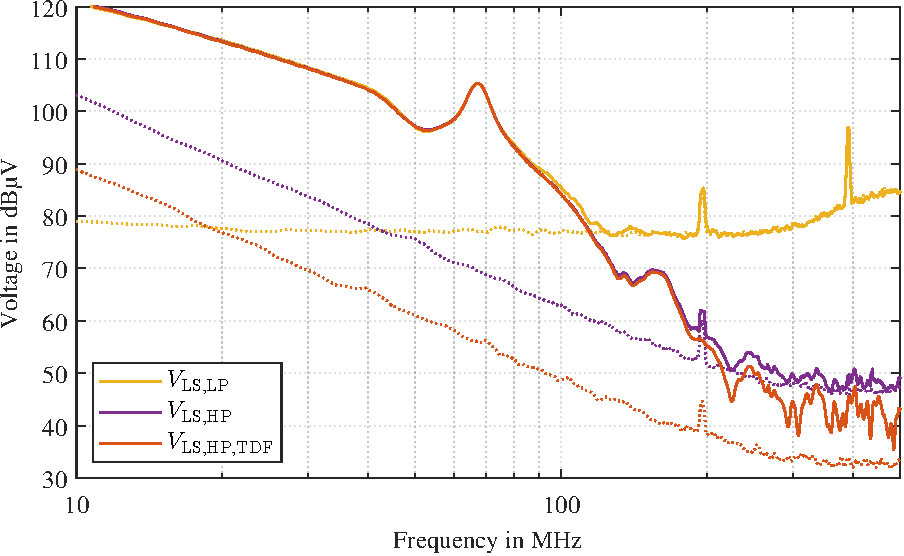
\includegraphics[scale = 1]{figures/7_MeasurementResults/MR_Methodology.pdf}
	\caption{Impact of different noise-reduction steps on the measurement (solid line) and the corresponding noise floor (dotted line).}\label{fig:MR_Methodology}
\end{figure}

Figure~\ref{fig:MR_Methodology} shows the spectrum used later, measured at the active low-side switch of an SiC MOSFET with an active area of \SI{5}{mm^2}, for the low-pass, high-pass, and TDF signals.
For each signal, two measurements are performed: one with DUT operation (signal of interest) and one background measurement without DUT operation to determine the noise floor, which is shown as a dotted line.
To evaluate both quantities in the same spectrum plot, the measured signals are compensated using the transfer functions in \eref{eq:HP_comp} and \eref{eq:TF_Shunt}.



In the low-pass spectrum, which corresponds to conventional measurements, the noise floor is around \SI{76}{dB\micro\volt}, which is sufficient for analyzing the switching transient up to \SI{115}{MHz}.
For higher frequencies, the signal falls below the noise level, which is why the high-pass measurement is necessary.

The high-pass measurement remains above the noise floor up to \SI{220}{MHz}, which is a significant improvement over the low-pass path.
However, the signal still decreases faster over frequency than the noise floor, so the SNR decreases at higher frequencies.
In the high-pass background measurement, the compensated noise floor decreases with frequency because the approximately constant noise measurement is divided by the increasing high-pass gain.

In a final step, the TDF filter is applied in post-processing, further reducing the noise floor by about \SI{15}{dB}.
This enables analysis of the switching transient up to \SI{500}{MHz}.





% \section{Demonstration of Switching Event Resolved Frequency Domain Analysis}
% In this section the switching event resolved frequency domain analysis is demonstrated, which provides a more detailed analysis of the noise contribution of the different switching events.
% The methodology is explained in detail in Section~\ref{subsec:SpectralSeparation}.
% The test results are for a first generation, Robert Bosch SiC MOSFET operated at $\mi{V}{DC} = \SI{800}{V}$, $\mi{I}{load} = \SI{60}{A} = \mi{I}{N,MOSFET}$, and $\mi{R}{G} = \SI{5.6}{\Omega}$, with a commutation-loop inductance of $\mi{L}{\sigma} = \SI{24}{nH}$ and an ambient temperature of $T = \SI{30}{\celsius}$.

% Figure~\ref{fig:MR_Demo_SpekSep_TD} shows the time-domain measurement results of the demonstration of switching event resolved frequency domain analysis.
% The two measured voltages of the active and passive switch are separated into the four artificial signals of the active-on, active-off, passive-on, and passive-off switching events.



% \begin{figure}[ht]
% 	\centering
% 	\begin{subfigure}[t]{\textwidth}
% 		\centering
% 		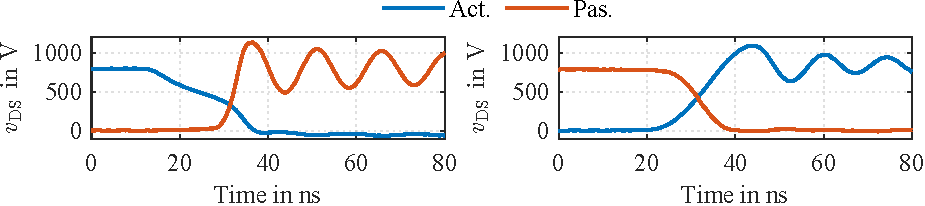
\includegraphics[scale = 1]{figures/6_Environment/MR_Demo_SpekSep/MR_Demo_SpekSep_ActPasVoltage_TD.pdf}
% 		\subcaption{Time-domain voltage measurement results of the active and passive switches.}
% 		\label{fig:MR_L_constE_Sweep_Voltage_TD}
% 	\end{subfigure} 
    
% 	\vspace{0.5cm}	
	
% 	\begin{subfigure}[t]{\textwidth}
% 		\centering
% 		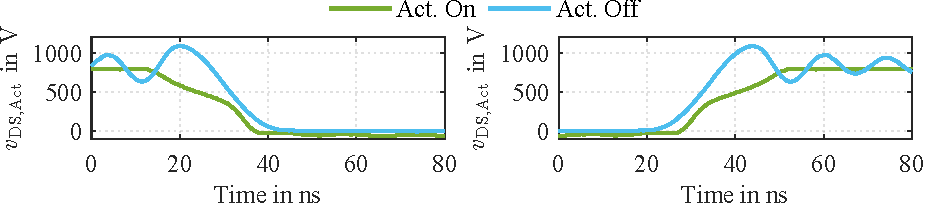
\includegraphics[scale = 1]{figures/6_Environment/MR_Demo_SpekSep/MR_Demo_SpekSep_ActVoltage_TD.pdf}
% 		\subcaption{Separated, artificial switching events of the active switch.}
% 		\label{fig:MR_L_constE_Sweep_ActVoltage_TD}
% 	\end{subfigure} 

% 	\vspace{0.5cm}

% 	\begin{subfigure}[t]{\textwidth}
% 		\centering
% 		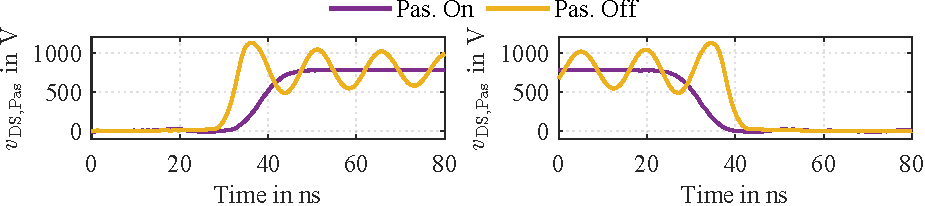
\includegraphics[scale = 1]{figures/6_Environment/MR_Demo_SpekSep/MR_Demo_SpekSep_PasVoltage_TD.pdf}
% 		\subcaption{Separated, artificial switching events of the passive switch.}
% 		\label{fig:MR_L_constE_Sweep_PasVoltage_TD}
% 	\end{subfigure} 

% 	\caption{Time-domain results of the demonstration of switching event resolved frequency domain analysis.}
% 	\label{fig:MR_Demo_SpekSep_TD}
% \end{figure}


% These measurements show the typical behavior of a MOSFET switched with a constant gate resistance at room temperature. 
% The observations can be summarized as follows:
% \begin{enumerate}
% 	\item The passive-off event exhibits a higher overvoltage than the active-off event (\SI{1130}{V} compared with \SI{1080}{V}), and this overvoltage increases with temperature because the body diode stores more bipolar charge.
% 	\item The passive-off event responds purely passively to the excitation transient, whereas the active-off event initially shows an approximately linear voltage increase controlled by the gate driver. This is followed by an inductive overshoot, only after which the output capacitance and the commutation-cell inductance begin to oscillate passively.
% 	\item The on-events also behave differently: the active-on event initially exhibits a voltage drop caused by the inductive voltage drop across the commutation-cell inductance, followed by the actual voltage commutation controlled by the gate driver. This creates two distinct transient times, and the faster or larger one dominates the spectrum.
% 	\item In contrast, the passive-on event shows a smooth voltage transient, which is the reaction of the passive $LC$ tank to the controlled active-off transient and is therefore smoothed by the impedance of the tank.
% \end{enumerate}

% These time-domain observations provide the physical basis for the event-resolved interpretation of the frequency-domain spectra. To understand the impact of the four distinct switching events on the measured spectrum, the same snap-and-mirror method is applied to the corresponding high-pass measurements and combined with the TDF filter in post-processing. The resulting frequency-domain results are shown in \fref{fig:MR_Demo_SpekSep_FD}.
% The general functionality of the snap-and-mirror method is demonstrated by the observation that, for both the active and passive switch emission spectra, one of the two contributing switching events (on or off) dominates specific frequency ranges, while the other contributes only marginally.

% \begin{figure}[!t]
% 	\centering
% 	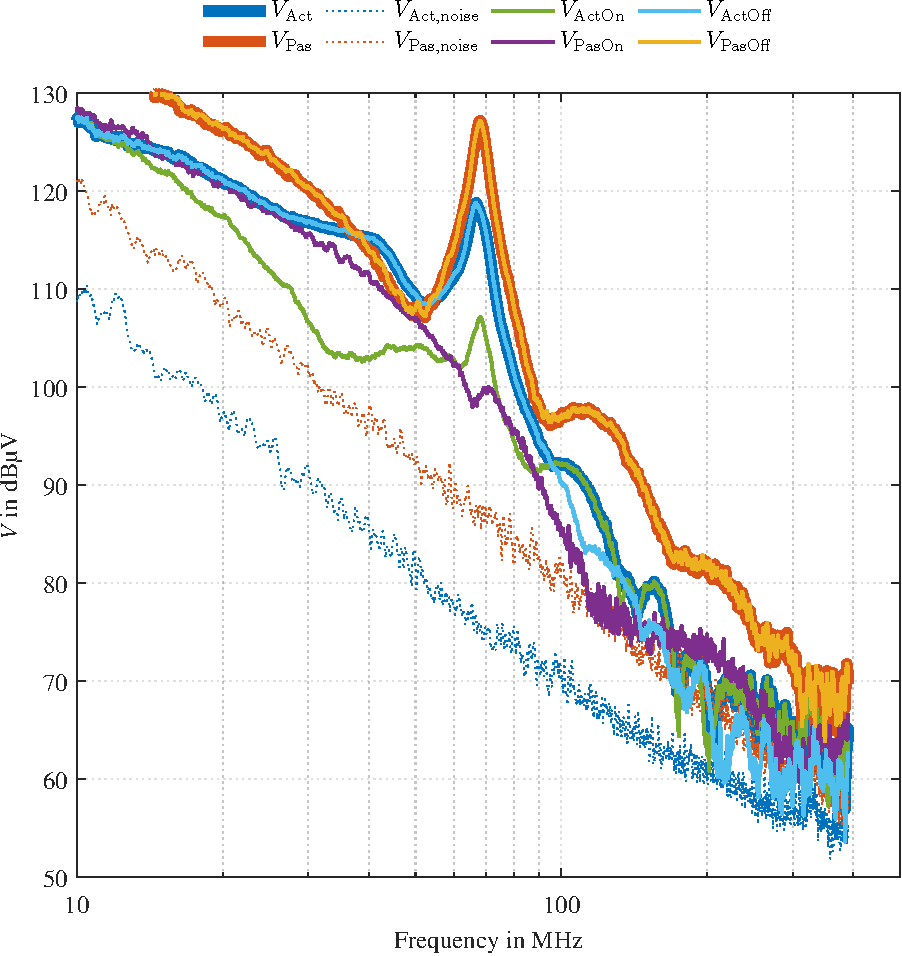
\includegraphics[scale = 1]{figures/6_Environment/MR_Demo_SpekSep/MR_Demo_SpekSep_FD.pdf}
% 	\caption{Frequency-domain measurement results of the demonstration of switching event resolved frequency domain analysis.}\label{fig:MR_Demo_SpekSep_FD}
% \end{figure}

% In addition, several consistent trends can be identified in the frequency-domain results over a wide range of operating conditions. These are summarized as follows:
% \begin{enumerate}
% 	\item The passive switch, and in particular the passive-off event, exhibits consistently higher emission than the active switch. This trend is consistent with the general EMC experience in the laboratory and is attributed to the larger overvoltage and stronger ringing of the passive switch.
% 	\item For the active switch, the turn-off event dominates the lower-frequency range and the resonance region; however, above approximately \SI{100}{MHz}, the turn-on event becomes dominant and reaches up to \SI{8}{dB} higher emission. The exact crossover frequency depends on the switching speed.
% 	\item A slight mismatch between the resonance frequencies of the active and passive switch is observed (\SI{66}{MHz} compared with \SI{69}{MHz}). 
% 	This difference increases for smaller chip sizes and lower capacitances, as predicted by the coupling model in \cite{liu_modeling_2016}. 
% 	The underlying cause is the different coupling of the oscillation into the gate loop of the active switch and the passive switch, respectively.
% 	\item A small resonance is observed in the active-on event, which is attributed to imperfect shielding and capacitive coupling from the passive-off event into the active-on contribution. 
% 	This effect is not observed in the passive-on event because the active-off event is significantly smaller in amplitude and therefore couples less strongly.
% 	\item Although the passive-on transient is faster than the active-on transient, its emission is lower in the high-frequency range. 
% 	This is due to the second, faster transient of the active-on event, which is steeper than the initial inductive voltage drop and therefore contributes more strongly to the high-frequency spectrum.
% 	\item The noise floor of the passive switch is higher than that of the active switch. 
% 	This is a consequence of the larger signal amplitude and the associated requirement for a larger vertical scale on the oscilloscope, which increases the measurement noise floor.
% \end{enumerate}

% Overall, the event-resolved analysis provides a detailed and physically transparent decomposition of the total noise emission into its dominant switching-event contributors. 
% This new method enables a much more precise assessment of the individual mechanisms that shape the measured spectrum and reveals which transient events actually limit the EMC performance at a given frequency range. In practical terms, this allows for targeted EMC debugging, since only the noisiest contributor determines the emission limit in a given frequency band. 
% As a result, optimization can be focused on the dominant source rather than on the total waveform, enabling faster or more aggressive switching of other contributors without increasing the total emitted noise. 
% This is particularly valuable for balancing switching losses and EMC performance, because the design space can be explored more deliberately when the limiting mechanism is known and not obscured by the aggregate signal.


%!TeX root = main.tex
%!encoding = UTF-8 Unicode

\section{LISN Measurement for System-Level Cross Reference}

This section presents the LISN measurements as a cross-reference to the intrinsic emission measurements.
As an example, a \SI{1200}{V} SiC MOSFET in a D2PAK package is used as the DUT, and the standard gate-resistance variation test is performed.
Since the oscilloscope ground is fixed to the aluminum base plate, no current measurement is carried out in this configuration.
The measurement results are shown in \fref{fig:MR_LISN_Voltage_TD} and \fref{fig:MR_LISN_LISN_TD} for the time domain and in \fref{fig:MR_LISN_FD} for the frequency domain.

\begin{figure}[ht]
	\centering
	\tikzsetnextfilename{MR_LISN_Voltage_TD}
	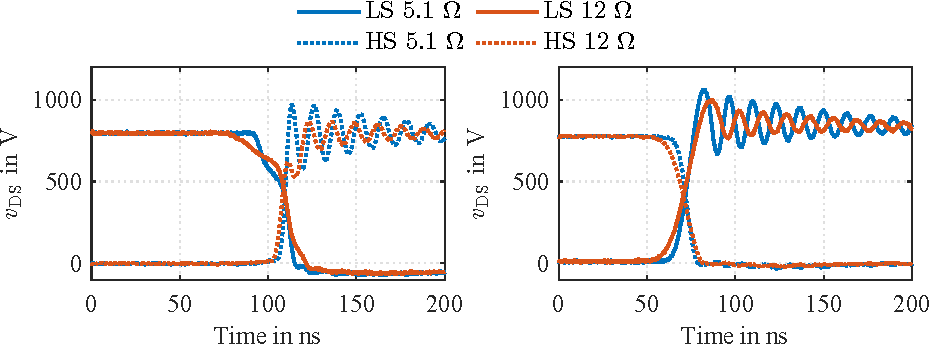
\includegraphics[scale=1]{figures/6_Environment/MR_LISN/MR_LISN_Voltage_TD.pdf}
	\caption{Time-domain measurement of low-side and high-side voltages for two gate resistances at \SI{800}{V} and \SI{60}{A} for PMTX03.}\label{fig:MR_LISN_Voltage_TD}
\end{figure}

\begin{figure}[ht]
	\centering
	\tikzsetnextfilename{MR_LISN_LISN_TD}
	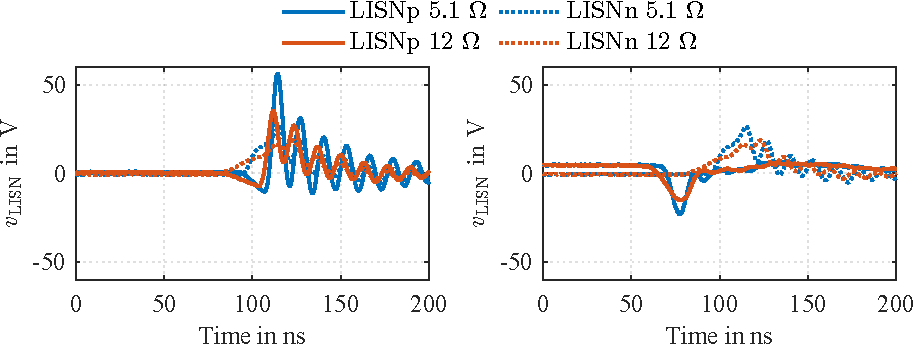
\includegraphics[scale=1]{figures/6_Environment/MR_LISN/MR_LISN_LISN_TD.pdf}
	\caption{Time-domain measurement of LISN voltages for two gate resistances at \SI{800}{V} and \SI{60}{A} for PMTX03.}\label{fig:MR_LISN_LISN_TD}
\end{figure}

The time-domain plots confirm the expected influence of increased gate resistance: the switching speed decreases and the voltage transitions become slower.
This is the classical behavior observed in gate-resistance variation studies.
In contrast, the frequency-domain plots provide more relevant information for EMC analysis, because they reveal how system-level parasitics and return paths shape the emission behavior.
These LISN measurements represent the state of the art for semiconductor-oriented EMC analysis, and their limitations are discussed in the following.

The upper graph of \fref{fig:MR_LISN_FD} shows the intrinsic emissions measured with the high-pass output of the DAVP.
The lower two graphs show the conventional LISN voltages, first directly and then in the translated common-mode and differential-mode components.
The corresponding voltages can be calculated as
\begin{equation}
    \mi{v}{CM} = \frac{1}{2}\cdot(\mi{v}{LISNp} + \mi{v}{LISNn})
\end{equation}

\begin{equation}
    \mi{v}{DM} = \frac{1}{2}\cdot(\mi{v}{LISNp} - \mi{v}{LISNn})
\end{equation}

When the LISN voltages are examined, the onset of the noise floor becomes evident slightly above the resonance frequency at \SI{75}{MHz}.
This noise floor is the same as the one introduced in Sec.~\ref{sec:MeasurementLimitation} and is only marginally lower than that of a direct drain-source voltage measurement, because the switching node couples capacitively to the cooler and then to the LISN terminals.
However, this creates a first-order transfer function, while the actual signal falls with second-order or even higher-order behavior.
This is clearly visible in the high-pass measurement of the drain-source voltages, which span a much wider range from \SI{40}{dB\mu V} to \SI{140}{dB\mu V}, compared to only about \SI{30}{dB} for the LISN voltages.
Consequently, the maximum measurable frequency in the system-level measurement with the LISN is approximately \SI{150}{MHz}, while the DAVP measures up to \SI{400}{MHz}.

\begin{figure}[ht]
	\centering
	\tikzsetnextfilename{MR_LISN_FD}
	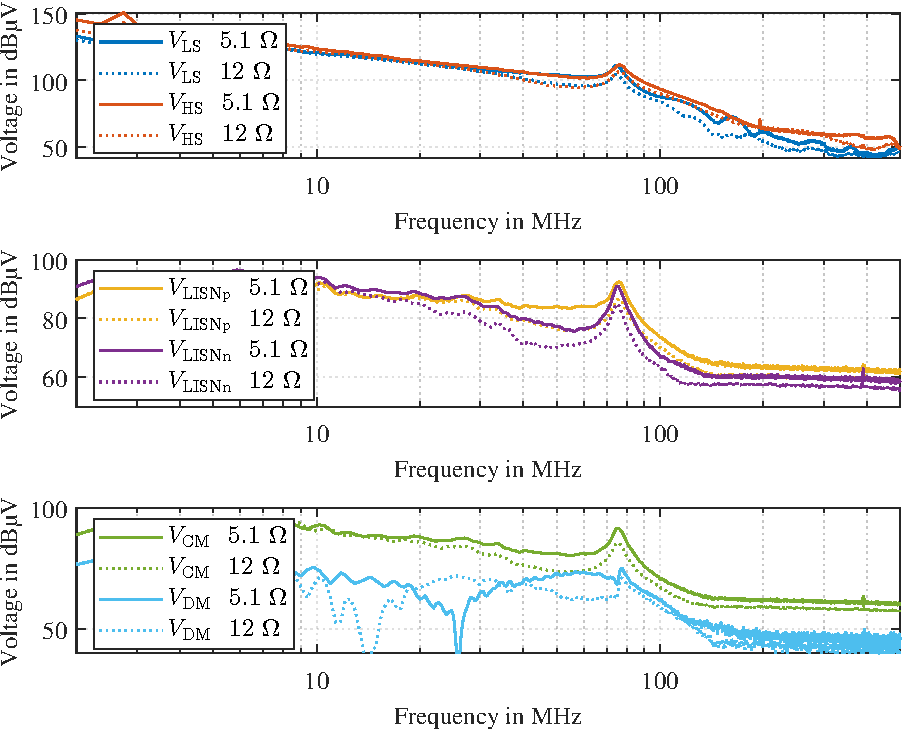
\includegraphics[scale=1]{figures/6_Environment/MR_LISN/MR_LISN_FD.pdf}
	\caption{Frequency-domain measurement of drain-source and LISN voltages for two gate resistances at \SI{800}{V} and \SI{60}{A} for PMTX03.}\label{fig:MR_LISN_FD}
\end{figure}

Nevertheless, some additional insight can be gained from the data.
When the high-side and low-side main resonances are compared, a small mismatch in resonance frequency becomes visible.
This is caused by passive turn-off, where the oscillation couples into the gate and the corresponding capacitances create a slight mismatch.
This effect does not occur during active turn-off, because the gate driver holds the gate capacitance constant.
This behavior is discussed in detail in \cite{paper}.
A similar mismatch can also be observed in the LISN voltages.
While the peak of \mi{v}{LISNp} occurs at \SI{76}{MHz}, the peak of \mi{v}{LISNn} occurs at \SI{74}{MHz}, which corresponds exactly to the resonances of \mi{v}{DS,HS} and \mi{v}{DS,LS}, respectively.
This can be explained by the positioning of the high-side and low-side MOSFETs relative to the positive and negative LISN terminals.
From \fref{fig:pic_b2b_setup}, it is evident that the high-side switch \mi{Q}{HS} is placed closer to LISNp, while \mi{Q}{LS} is placed closer to LISNn.
The respective noise of each switch therefore follows the lowest-impedance or shortest return path.
Furthermore, the general slope of the raw emission \mi{v}{DS} is also visible in the system-level measurements \mi{v}{LISN}, confirming the validity of the complete measurement approach.

In future work, the transfer function between these two measurement types should be investigated.
This would enable system-level information to be extracted from raw emission measurements and extend the usable range of this approach.






%!TeX root = main.tex
%!encoding = UTF-8 Unicode

\section{Demonstration of Switching Event Resolved Frequency Domain Analysis}
In this section the switching event resolved frequency domain analysis is demonstrated, which provides a more detailed analysis of the noise contribution of the different switching events.
The methodology is explained in detail in Section~\ref{subsec:SpectralSeparation}.
The test results are for a first generation, Robert Bosch SiC MOSFET operated at $\mi{V}{DC} = \SI{800}{V}$, $\mi{I}{load} = \SI{60}{A} = \mi{I}{N,MOSFET}$, and $\mi{R}{G} = \SI{5.6}{\Omega}$, with a commutation-loop inductance of $\mi{L}{\sigma} = \SI{24}{nH}$ and an ambient temperature of $T = \SI{30}{\celsius}$.

Figure~\ref{fig:MR_Demo_SpekSep_TD} shows the time-domain measurement results of the demonstration of switching event resolved frequency domain analysis.
The two measured voltages of the active and passive switch are separated into the four artificial signals of the active-on, active-off, passive-on, and passive-off switching events.



\begin{figure}[ht]
	\centering
	\begin{subfigure}[t]{\textwidth}
		\centering
		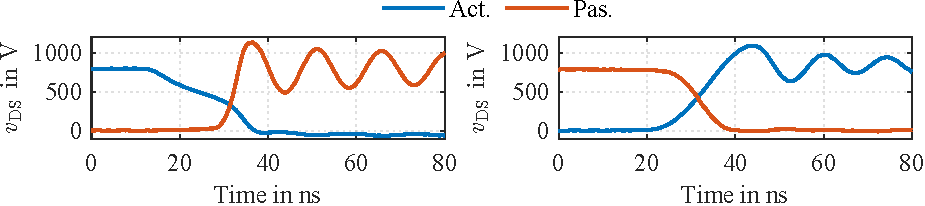
\includegraphics[scale = 1]{figures/6_Environment/MR_Demo_SpekSep/MR_Demo_SpekSep_ActPasVoltage_TD.pdf}
		\subcaption{Time-domain voltage measurement results of the active and passive switches.}
		\label{fig:MR_Demo_SpekSep_Voltage_TD}
	\end{subfigure} 
    
	\vspace{0.5cm}	
	
	\begin{subfigure}[t]{\textwidth}
		\centering
		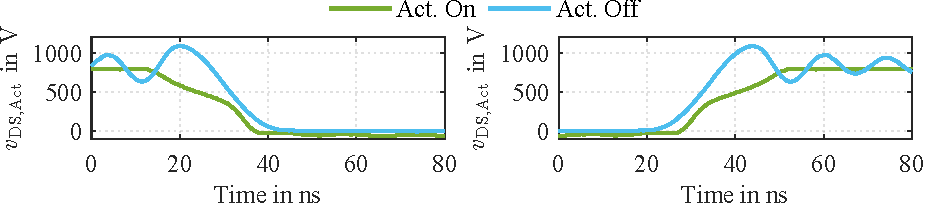
\includegraphics[scale = 1]{figures/6_Environment/MR_Demo_SpekSep/MR_Demo_SpekSep_ActVoltage_TD.pdf}
		\subcaption{Separated, artificial switching events of the active switch.}
		\label{fig:MR_Demo_SpekSep_ActVoltage_TD}
	\end{subfigure} 

	\vspace{0.5cm}

	\begin{subfigure}[t]{\textwidth}
		\centering
		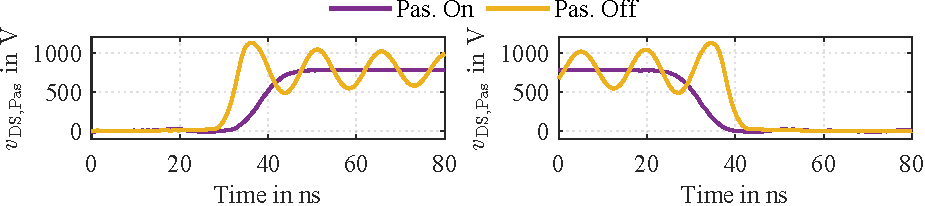
\includegraphics[scale = 1]{figures/6_Environment/MR_Demo_SpekSep/MR_Demo_SpekSep_PasVoltage_TD.pdf}
		\subcaption{Separated, artificial switching events of the passive switch.}
		\label{fig:MR_Demo_SpekSep_PasVoltage_TD}
	\end{subfigure} 

	\caption{Time-domain results of the demonstration of switching event resolved frequency domain analysis.}
	\label{fig:MR_Demo_SpekSep_TD}
\end{figure}


These measurements show the typical behavior of a MOSFET switched with a constant gate resistance at room temperature. 
The observations can be summarized as follows:
\begin{enumerate}
	\item The passive-off event exhibits a higher overvoltage than the active-off event (\SI{1130}{V} compared with \SI{1080}{V}), and this overvoltage increases with temperature because the body diode stores more bipolar charge.
	\item The passive-off event responds purely passively to the excitation transient, whereas the active-off event initially shows an approximately linear voltage increase controlled by the gate driver. This is followed by an inductive overshoot, only after which the output capacitance and the commutation-cell inductance begin to oscillate passively.
	\item The on-events also behave differently: the active-on event initially exhibits a voltage drop caused by the inductive voltage drop across the commutation-cell inductance, followed by the actual voltage commutation controlled by the gate driver. This creates two distinct transient times, and the faster or larger one dominates the spectrum.
	\item In contrast, the passive-on event shows a smooth voltage transient, which is the reaction of the passive $LC$ tank to the controlled active-off transient and is therefore smoothed by the impedance of the tank.
\end{enumerate}

These time-domain observations provide the physical basis for the event-resolved interpretation of the frequency-domain spectra. To understand the impact of the four distinct switching events on the measured spectrum, the same snap-and-mirror method is applied to the corresponding high-pass measurements and combined with the TDF filter in post-processing. The resulting frequency-domain results are shown in \fref{fig:MR_Demo_SpekSep_FD}.
The general functionality of the snap-and-mirror method is demonstrated by the observation that, for both the active and passive switch emission spectra, one of the two contributing switching events (on or off) dominates specific frequency ranges, while the other contributes only marginally.

\begin{figure}[!t]
	\centering
	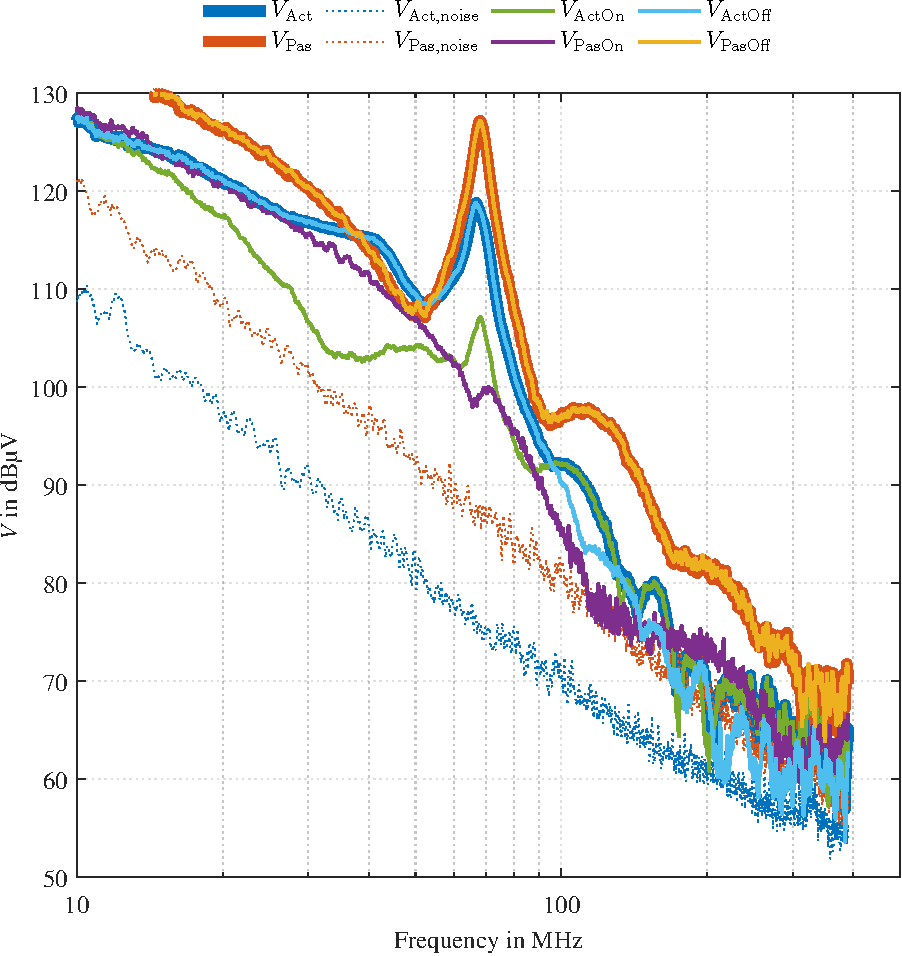
\includegraphics[scale = 1]{figures/6_Environment/MR_Demo_SpekSep/MR_Demo_SpekSep_FD.pdf}
	\caption{Frequency-domain measurement results of the demonstration of switching event resolved frequency domain analysis.}\label{fig:MR_Demo_SpekSep_FD}
\end{figure}

In addition, several consistent trends can be identified in the frequency-domain results over a wide range of operating conditions. These are summarized as follows:
\begin{enumerate}
	\item The passive switch, and in particular the passive-off event, exhibits consistently higher emission than the active switch. This trend is consistent with the general EMC experience in the laboratory and is attributed to the larger overvoltage and stronger ringing of the passive switch.
	\item For the active switch, the turn-off event dominates the lower-frequency range and the resonance region; however, above approximately \SI{100}{MHz}, the turn-on event becomes dominant and reaches up to \SI{8}{dB} higher emission. The exact crossover frequency depends on the switching speed.
	\item A slight mismatch between the resonance frequencies of the active and passive switch is observed (\SI{66}{MHz} compared with \SI{69}{MHz}). 
	This difference increases for smaller chip sizes and lower capacitances, as predicted by the coupling model in \cite{liu_modeling_2016}. 
	The underlying cause is the different coupling of the oscillation into the gate loop of the active switch and the passive switch, respectively.
	\item A small resonance is observed in the active-on event, which is attributed to imperfect shielding and capacitive coupling from the passive-off event into the active-on contribution. 
	This effect is not observed in the passive-on event because the active-off event is significantly smaller in amplitude and therefore couples less strongly.
	\item Although the passive-on transient is faster than the active-on transient, its emission is lower in the high-frequency range. 
	This is due to the second, faster transient of the active-on event, which is steeper than the initial inductive voltage drop and therefore contributes more strongly to the high-frequency spectrum.
	\item The noise floor of the passive switch is higher than that of the active switch. 
	This is a consequence of the larger signal amplitude and the associated requirement for a larger vertical scale on the oscilloscope, which increases the measurement noise floor.
\end{enumerate}

Overall, the event-resolved analysis provides a detailed and physically transparent decomposition of the total noise emission into its dominant switching-event contributors. 
This new method enables a much more precise assessment of the individual mechanisms that shape the measured spectrum and reveals which transient events actually limit the EMC performance at a given frequency range. In practical terms, this allows for targeted EMC debugging, since only the noisiest contributor determines the emission limit in a given frequency band. 
As a result, optimization can be focused on the dominant source rather than on the total waveform, enabling faster or more aggressive switching of other contributors without increasing the total emitted noise. 
This is particularly valuable for balancing switching losses and EMC performance, because the design space can be explored more deliberately when the limiting mechanism is known and not obscured by the aggregate signal.



\section{Characterization of the Intrinsic SiC MOSFET Emissions}
\label{sec:Results}

As the final step of this thesis, this chapter presents measurement results obtained with the measurement methodology introduced in Chapter~\ref{ch:Methods} and the experimental setup described in Sections~\ref{ch:voltage} and~\ref{ch:AShunt}.
Since a wide range of parameters can be investigated with the proposed setup, this chapter focuses on the subset that is most instructive for the reader and most relevant to circuit design practice.
These parameters are separated into external parameters, which are set by the application engineer, and MOSFET parameters, which are set by the device engineer.
To draw a fair conclusion about the influence of each parameter, the comparison must be performed under a well-defined measurement constraint, because the emissions otherwise depend on multiple, correlated quantities simultaneously.
Depending on the use case, the influence of a parameter under constant gate resistance, constant maximum overvoltage, or constant switching losses is of interest.
While the complete set of measurements is documented in Appendix~\ref{app:additional_measurements}, only the comparisons obtained under constant switching losses are discussed in the main text for the sake of conciseness, as this constraint reflects the most common design target in practice.

The remainder of this chapter is structured as follows: Section~\ref{sec:MR_External} discusses the influence of external parameters, Section~\ref{sec:MR_MOSFET} discusses the influence of MOSFET parameters, and, lastly, Section~\ref{sec:MR_Summary} condenses the results under a given spectral FOM into a summary table that allows for a direct comparison of the influence of each parameter on the EM emissions.

Except otherwise stated, the measurement conditions are stated in \tref{tab:MR_conditions}.

\begin{table}[ht]
	\caption{Default electrical measurement conditions. Unless a parameter is the subject of the sweep in a given subsection, it is set to the value stated here.}
	\label{tab:MR_conditions}
	\centering
	\begin{tabular}{@{}llc@{}}
		\toprule
		\textbf{Parameter} & \textbf{Symbol} & \textbf{Value} \\
		\midrule
		DC-link voltage & \mi{V}{DC} & \SI{800}{V} \\
		Load current & \mi{I}{L} & \SI{60}{A} \\
		Device blocking-voltage rating & \mi{V}{(BR)DSS} & \SI{1200}{V} \\
		Device current rating & \mi{I}{D} & \SI{60}{A} \\
		Package & -- & D2PAK \\
		Commutation-loop inductance & \mi{L}{\sigma} & \SI{24}{nH} \\
		Negative gate-driver bias & \mi{V}{EE} & \SI{-5}{V} \\
		Positive gate-driver bias & \mi{V}{DD} & \SI{18}{V} \\
		Ambient temperature & \mi{T}{amb} & room temperature ($\approx$\SI{25}{\celsius}) \\
		\bottomrule
	\end{tabular}
\end{table}


%!TeX root = main.tex
%!encoding = UTF-8 Unicode
\subsection{Influence of External Parameters}
\label{sec:MR_External}

This section examines the influence of parameters that are accessible to the application engineer without altering the MOSFET itself, namely the gate resistance, the negative gate-driver bias, the junction temperature, and the commutation-loop inductance.
These parameters are routinely tuned during converter design to trade off switching losses, overvoltage, and electromagnetic interference, which makes their individual impact on the intrinsic EM emissions particularly relevant for practical converter design.
For each parameter, a sweep is performed while the switching losses are kept constant (except the gate resistance), so that the differences observed in the frequency-domain spectra can be attributed to the parameter itself rather than to a shift in the switching speed.
Unless the parameter under study in a given subsection dictates otherwise, all remaining measurement conditions are set to the default values listed in Table~\ref{tab:MR_conditions}.
The four parameters are discussed in the order given above, starting with the gate resistance and the negative gate-driver bias, which shape the switching transient directly through the gate loop, followed by the junction temperature, which alters the intrinsic properties of the device itself, and concluding with the commutation-loop inductance, which is set by the layout of the power stage rather than by the device or its driver.

\subsubsection*{Gate Resistance}

The most common and straightforward way to control the switching speed of a MOSFET is to adjust the gate resistance.
By increasing the external gate resistance, the time constant formed with the gate-source and gate-drain capacitances increases, which slows down both the voltage and current switching transients and, thereby, also decreases the EM emissions.
However, this comes at the cost of increased switching losses, which is why the gate resistance is often tuned to achieve a trade-off between switching losses and EM emissions.
Note that the gate resistance does not directly damp the commutation-loop resonance, since it is not part of the resonant tank formed by the commutation-loop inductance and the device output capacitance; instead, it reduces the \mi{dv}{dt} and \mi{di}{dt} of the switching transient itself, which lowers the excitation of that resonance and, as a consequence, also its observed overshoot and ringing amplitude.

\begin{figure}[!ht]
	\centering
	\begin{subfigure}[t]{\textwidth}
		\centering
		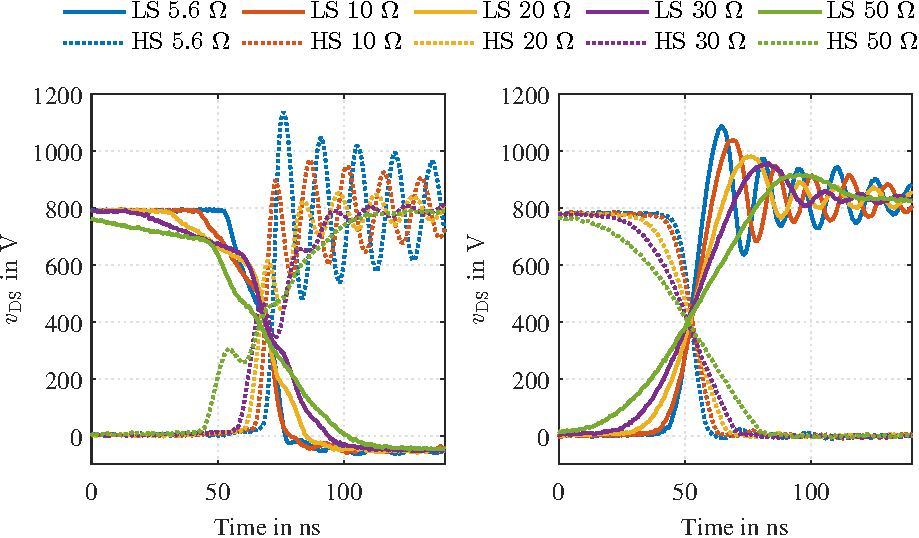
\includegraphics[scale = 1]{figures/7_MeasurementResults/MR_Rg/MR_Rg_Voltage_TD.pdf}
		\subcaption{Time-domain voltage measurement results.}
		\label{fig:MR_Rg_Sweep_Voltage_TD}
	\end{subfigure} 
    
	\vspace{0.5cm}	
	
    \begin{subfigure}[t]{\textwidth}
		\centering
		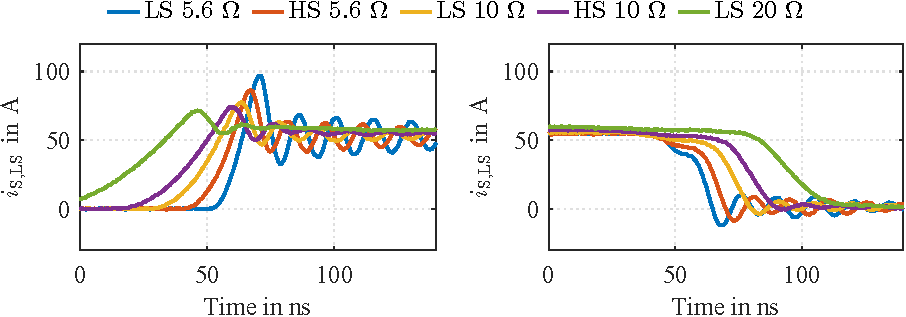
\includegraphics[scale = 1]{figures/7_MeasurementResults/MR_Rg/MR_Rg_Current_TD.pdf}
		\subcaption{Time-domain current measurement results.}
		\label{fig:MR_Rg_Sweep_Current_TD}
	\end{subfigure}
	\caption{Time-domain results of the gate-resistance sweep.}
	\label{fig:MR_Rg_Sweep_TD}
\end{figure}

The structure of the presented measurement results is the same for all external parameters: First, the time-domain voltage and current waveforms are shown, followed by the frequency-domain spectra.
Here, the solid lines are the low-side device, which is for all measurements the active device, and the dashed lines are the high-side device, which is for all measurements the passive device.
Then, the EM emissions are plotted against the switching losses to illustrate the trade-off between these two quantities.
Finally, the EM emissions are separated for turn-on and turn-off to highlight the differences in the emission behavior of these two switching events.

The time-domain results of the gate resistance, shown in Fig.~\ref{fig:MR_Rg_Sweep_TD}, show the expected and well-known trend.
By increasing the gate resistance from \SI{5.6}{\Omega} to \SI{50}{\Omega}, the switching speed is slowed down by a factor of approximately 10.
This factor is only slightly shifted by the MOSFET's internal gate resistance of \SI{3.5}{\Omega} (taken from the device datasheet), which adds to the total gate resistance.
In addition to the reduced switching speed, the overvoltage and the excited main resonance of the commutation-loop inductance and the output capacitance of the turned-off device are also reduced, which is a direct consequence of the reduced excitation through the switching transient.

\begin{figure}[ht]
	\centering
	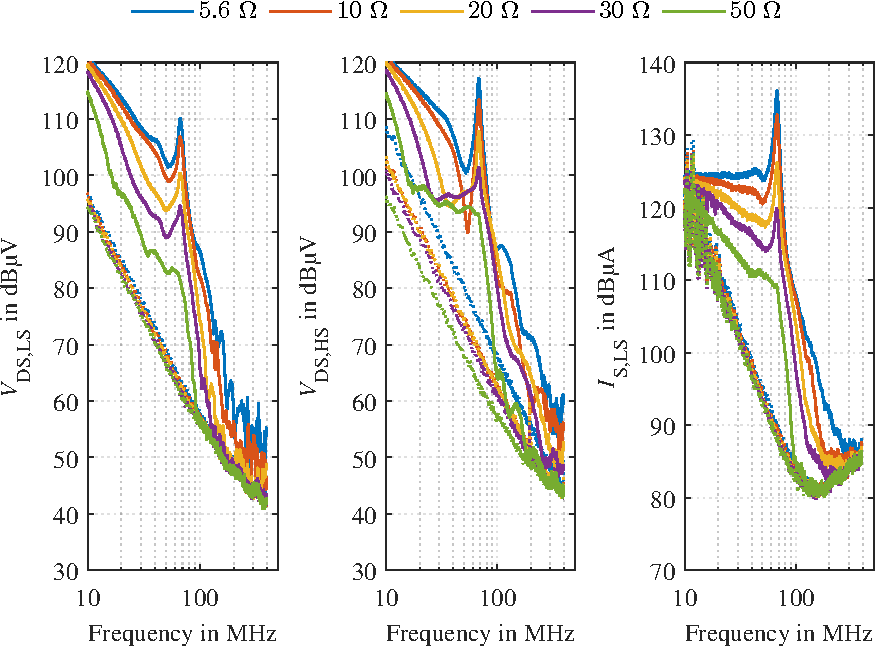
\includegraphics[scale = 1]{figures/7_MeasurementResults/MR_Rg/MR_Rg_FD.pdf}
	\caption{Frequency-domain measurement results of gate resistance sweep.}\label{fig:MR_Rg_Sweep_FD}
\end{figure}

The influence of the gate resistance on the emission spectrum is shown in \fref{fig:MR_Rg_Sweep_FD}, separated for the active and passive device and the commutation current.
Due to the reduced switching speed the entire spectrum is shifted towards lower frequencies, which is a direct consequence of the reduced slew rate of the switching transient.
Additionally, because the switching transient is slowed down, the amplitude of the excited main resonance is also reduced, to the point of no longer being clearly visible for \SI{50}{\Omega}.

To quantify the influence of the gate resistance on the EM emissions the spectral average FOM is used, which describes the average emissions for a given frequency range from \SI{30}{\mega\hertz} to \SI{200}{\giga\hertz}.
Here, caution must be taken, because for the highest gate-resistance measurements, the signal in the active device becomes so low that it falls below the noise floor earlier.
Hence, the average FOM is biased: it shows a higher value and thus indicates less sensitivity at higher gate resistances.
This effect is a direct consequence of the fundamental measurement noise floor discussed in Section~\ref{sec:MeasurementLimitation}, and it must be kept in mind whenever the average FOM is compared between measurements with strongly differing emission levels, as is the case here for the lowest and the highest gate resistance.

\begin{figure}[ht]
	\centering
	\begin{subfigure}[t]{\textwidth}
		\centering
		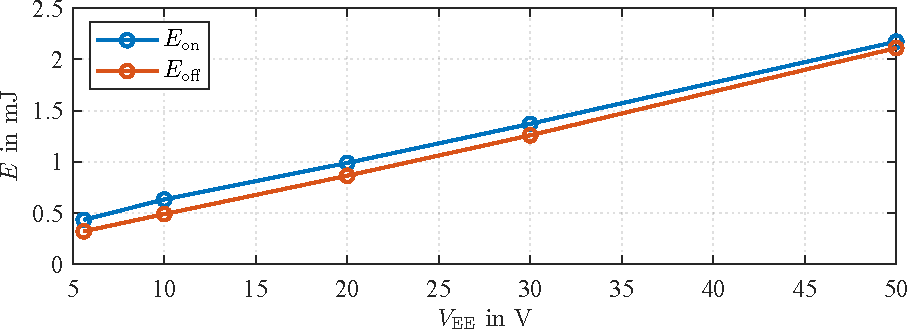
\includegraphics[scale = 1]{figures/7_MeasurementResults/MR_Rg/MR_Rg_Losses.pdf}
		\subcaption{Influence of gate resistance and switching losses on the EM emissions.}
		\label{fig:MR_Rg_EmissionOverLosses}
	\end{subfigure} 

	\vspace{0.5cm}
	
    \begin{subfigure}[t]{\textwidth}
		\centering
		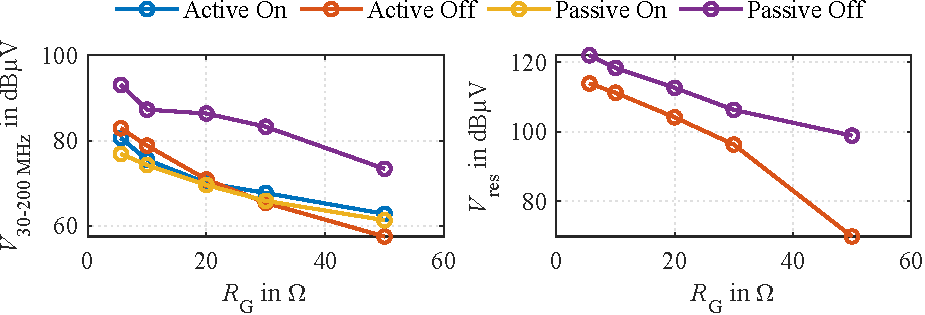
\includegraphics[scale = 1]{figures/7_MeasurementResults/MR_Rg/MR_Rg_Emission.pdf}
		\subcaption{EM emissions separated for turn-on and turn-off.}
		\label{fig:MR_Rg_Emission}
	\end{subfigure}
	\caption{Gate-resistance-dependent emission and loss analysis.}
\end{figure}

The influence of the gate resistance on the switching losses and the EM emissions is shown in \fref{fig:MR_Rg_EmissionOverLosses} and \fref{fig:MR_Rg_Emission}, where the average FOM is plotted against the gate resistance.
Here, the snap-and-mirror function is used to separate the influence of the gate resistance onto the four switching transients, as described in Section~\ref{subsec:SpectralSeparation}.
The analysis shows, in addition to the spectral average, the resonance peak value of the main resonance.
Since the gate resistance has the same impact on all switching transients, the spectrum shows the same trend for all events, only offset by the general emission level of the switching event.
When assumed linearly, an influence of \SI{-0.5}{dB/\Omega} can be derived for the gate resistance on the average FOM, which is a significant influence, especially when compared to the other external parameters discussed in this section.
For the converter designer, this sensitivity means that, within the limits set by the acceptable switching losses, tuning the gate resistance remains the single most effective lever among the four parameters discussed in this section for trading off EM emissions against switching speed, whereas the remaining parameters, discussed next, offer comparatively smaller but often loss-free means of fine-tuning the emission spectrum.

\FloatBarrier

\subsubsection*{Negative Gate-Driver Bias}

Besides the gate resistance, the negative gate-driver bias \mi{V}{EE} provides a second, independent means to shape the switching transients.
Increasing the magnitude of the negative bias raises the negative overdrive voltage applied to the gate, thereby increasing the driving voltage across the gate loop during turn-off and, consequently, the achievable turn-off speed.
At the same time, a larger negative bias widens the voltage span across which the gate-loop inductance must be charged when the device is switched back on, from \mi{V}{EE} up to the threshold voltage, which prolongs the charging time of the gate loop and thereby delays the onset of the subsequent turn-on transient.
The negative gate-driver bias further affects the freewheeling body diode: as the gate voltage is driven closer to zero, less bipolar charge is stored in the intrinsic body diode, because a less negative bias increasingly allows unipolar channel conduction to contribute to the freewheeling current instead of the diode alone.
The negative gate-driver bias is therefore expected to influence the turn-off- and turn-on-related emissions, as well as the reverse-recovery-related emissions of the freewheeling diode.

\begin{figure}[ht]
	\centering
	\begin{subfigure}[t]{\textwidth}
		\centering
		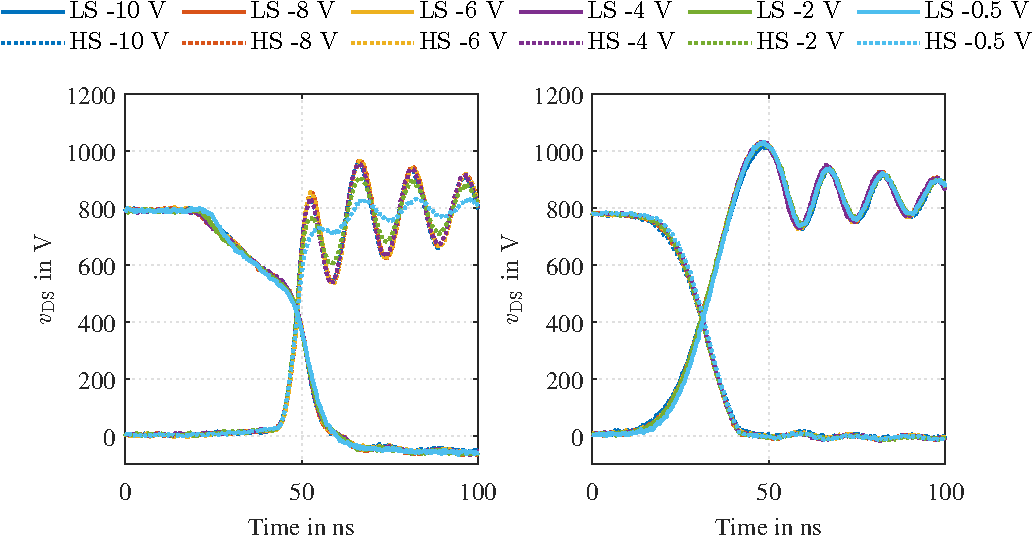
\includegraphics[scale = 1]{figures/7_MeasurementResults/MR_Vee_constE/MR_Vee_constE_Voltage_TD.pdf}
		\subcaption{Time-domain voltage measurement results.}
		\label{fig:MR_Vee_constE_Sweep_Voltage_TD}
	\end{subfigure} 
    
	\vspace{0.5cm}

    \begin{subfigure}[t]{\textwidth}
		\centering
		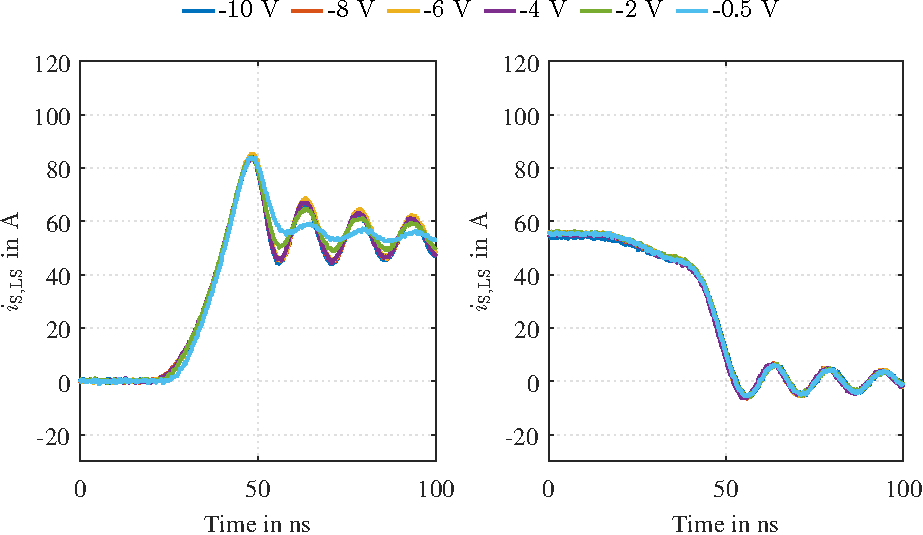
\includegraphics[scale = 1]{figures/7_MeasurementResults/MR_Vee_constE/MR_Vee_constE_Current_TD.pdf}
		\subcaption{Time-domain current measurement results.}
		\label{fig:MR_Vee_constE_Sweep_Current_TD}
	\end{subfigure}
	\caption{Time-domain results of the negative gate-driver bias sweep.}
	\label{fig:MR_Vee_constE_Sweep_TD}
\end{figure}

Fig.~\ref{fig:MR_Vee_constE_Sweep_TD} shows the time-domain results of the negative-gate-driver-bias sweep, covering the range from \SI{-10}{V} to \SI{-0.5}{V}.
Throughout this sweep, the gate resistance is co-adjusted to keep the switching losses constant; as a consequence, the active-off transient, whose speed is governed exclusively by this compensated gate resistance, remains unaffected by the change in bias.
In contrast, a clear influence is observed for the active-on and passive-off transients: between \SI{-10}{V} and \SI{-4}{V} this influence remains minor, whereas for \SI{-2}{V} and \SI{-0.5}{V} the passive switch increasingly loses its resonant ringing behavior.
This trend is consistent with the reduced bipolar charge in the freewheeling diode as the gate bias becomes less negative.


\begin{figure}[ht]
	\centering
	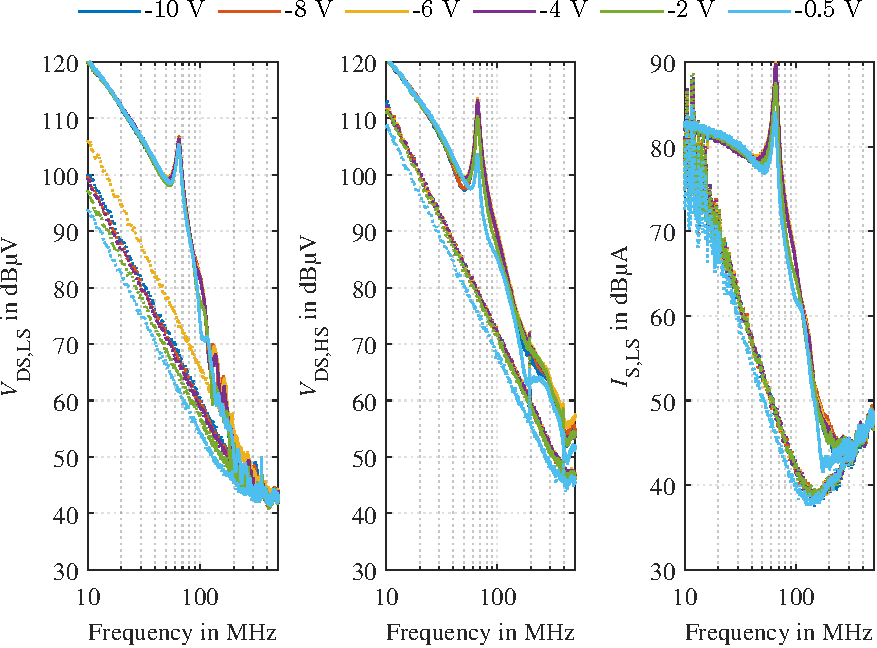
\includegraphics[scale = 1]{figures/7_MeasurementResults/MR_Vee_constE/MR_Vee_constE_FD.pdf}
	\caption{Frequency-domain measurement results of negative gate-driver bias sweep.}\label{fig:MR_Vee_constE_Sweep_FD}
\end{figure}

The corresponding frequency-domain spectra, shown in \fref{fig:MR_Vee_constE_Sweep_FD} and again separated for the active and passive device as well as the commutation current, confirm this trend.
No discernible influence of the negative gate-driver bias is observed in the voltage spectrum between \SI{-10}{V} and \SI{-4}{V}, whereas for \SI{-2}{V} and \SI{-0.5}{V} the main resonance of the passive device is increasingly suppressed and the broadband emissions decrease as a result of the smoother transient.

\begin{figure}[ht]
	\centering
	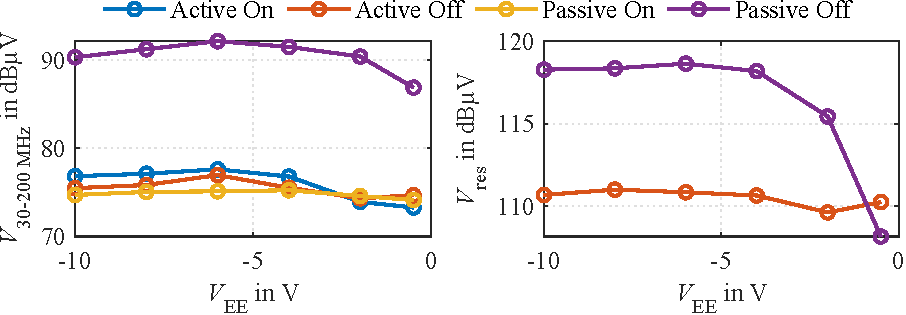
\includegraphics[scale = 1]{figures/7_MeasurementResults/MR_Vee_constE/MR_Vee_constE_Emission.pdf}
	\caption{Influence of the negative gate-driver bias on the EM emission.}\label{fig:MR_Vee_constE_Emission}
\end{figure}

This behavior is quantified in \fref{fig:MR_Vee_constE_Emission}, where the average FOM is plotted against the negative gate-driver bias.
While the active-off and passive-on transients show virtually no dependency, the active-on and passive-off transients exhibit a clear trend: from \SI{-4}{V} to \SI{-0.5}{V} the average FOM decreases by \SI{5}{dB}, a significant influence compared to the other external parameters discussed in this section, and the passive-off resonance peak is damped even more strongly, by \SI{10.5}{dB}.

\FloatBarrier

\subsubsection*{Junction Temperature}

The junction temperature affects several device properties that can be relevant for the switching behavior of the MOSFET, namely the amount of bipolar charge stored in the intrinsic body diode, the threshold voltage \mi{V}{th}, and the internal gate resistance \mi{R}{g,int}.
With increasing temperature, the minority-carrier lifetime in the body diode increases, so that more bipolar charge is stored during freewheeling conduction; upon commutation, this additional charge must be removed as reverse-recovery charge, which is expected to increase the reverse-recovery current peak and to prolong the current tail of the freewheeling device.
The threshold voltage of the SiC MOSFET decreases with increasing temperature, which shifts the gate-source voltage at which channel conduction sets in, thereby speeding up the turn-on and slowing down the turn-off.
The internal gate resistance, in turn, increases with temperature due to the positive temperature coefficient of the polysilicon gate material, which would, on its own, slow down the switching transient.
Since the external gate resistance is co-adjusted in this sweep to keep the switching losses constant, the direct influence of \mi{V}{th} and \mi{R}{g,int} on the switching speed is largely compensated, so that the remaining, temperature-dependent differences in the spectra are expected to be dominated by the reverse-recovery behavior of the freewheeling diode, i.e., the turn-on-related and diode-related emissions.

\begin{figure}[ht]
	\centering
	\begin{subfigure}[t]{\textwidth}
		\centering
		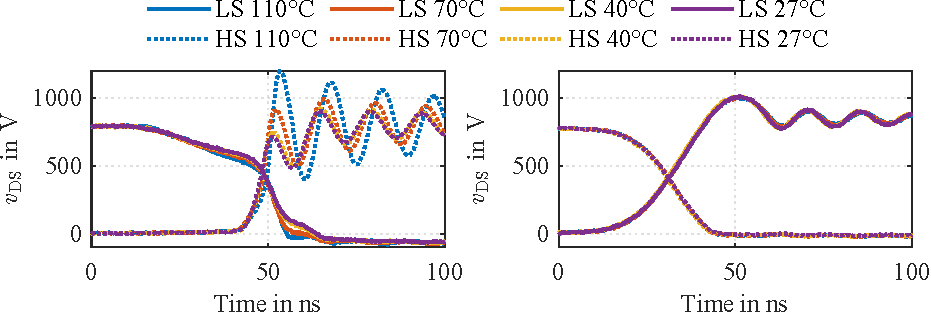
\includegraphics[scale = 1]{figures/7_MeasurementResults/MR_T_constE/MR_T_constE_Voltage_TD.pdf}
		\subcaption{Time-domain voltage measurement results.}
		\label{fig:MR_T_constE_Sweep_Voltage_TD}
	\end{subfigure} 
    
	\vspace{0.5cm}	
	
    \begin{subfigure}[t]{\textwidth}
		\centering
		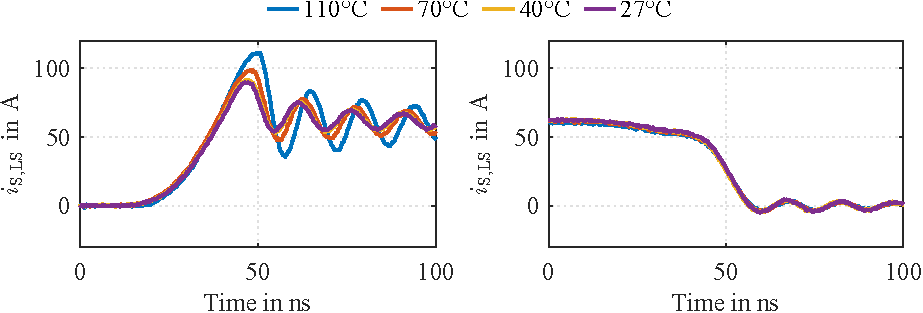
\includegraphics[scale = 1]{figures/7_MeasurementResults/MR_T_constE/MR_T_constE_Current_TD.pdf}
		\subcaption{Time-domain current measurement results.}
		\label{fig:MR_T_constE_Sweep_Current_TD}
	\end{subfigure}
	\caption{Time-domain results of the case-temperature sweep.}
	\label{fig:MR_T_constE_Sweep_TD}
\end{figure}

It must be noted that, in this measurement, the device under test is heated externally from the top of the D2PAK package rather than through the switching losses themselves; consequently, the temperature stated for this sweep, \mi{T}{case}, is a case temperature rather than the junction temperature \mi{T}{j}.
Because the chip is located at the bottom of the package and is thermally connected to the PCB copper acting as a heat sink, the actual junction temperature may be somewhat lower than the stated case temperature.
The presented temperature dependency should therefore be interpreted qualitatively as a lower bound on the true sensitivity to the junction temperature.
Additionally, the maximum temperature is limited by the maximum power rating of the meander structure used; the semiconductor chip itself could be operated at a much higher temperature of at least \SI{175}{\celsius}.

Fig.~\ref{fig:MR_T_constE_Sweep_TD} shows the time-domain results of the case-temperature sweep, covering the range from \SI{27}{\celsius} to \SI{110}{\celsius}.
The turn-off transient, i.e., the active-off and passive-on switching event, is virtually unaffected by the case temperature: the voltage and current waveforms of all four temperatures overlap almost perfectly.
In contrast, a pronounced temperature dependence is visible for the turn-on transient, i.e., the active-on and passive-off switching event: with increasing case temperature, the reverse-recovery current peak of the freewheeling device increases noticeably, from approximately \SI{89}{\ampere} at \SI{27}{\celsius} to approximately \SI{112}{\ampere} at \SI{110}{\celsius},
and the associated voltage overshoot and ringing of the passive device likewise increase with temperature.
This behavior is consistent with the increased bipolar charge stored in the body diode at elevated temperatures, which must be removed during commutation and thereby increases both the reverse-recovery current and the excitation of the commutation-loop resonance.

\begin{figure}[ht]
	\centering
	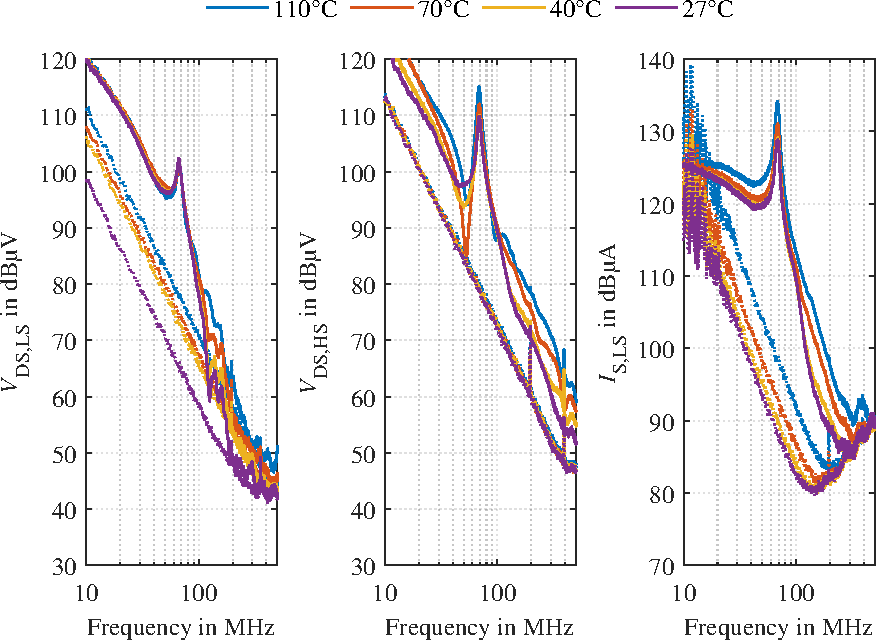
\includegraphics[scale = 0.95]{figures/7_MeasurementResults/MR_T_constE/MR_T_constE_FD.pdf}
	\caption{Frequency-domain measurement results of case-temperature sweep.}\label{fig:MR_T_constE_Sweep_FD}
\end{figure}

The corresponding frequency-domain spectra are shown in \fref{fig:MR_T_constE_Sweep_FD}, separated for the active and passive device and the commutation current.
Across the entire frequency range, the spectra obtained at \SI{27}{\celsius} and \SI{40}{\celsius} lie visibly below those obtained at \SI{70}{\celsius} and \SI{110}{\celsius}, and the resonance peak located around \SI{70}{\mega\hertz}, which is excited by the reverse-recovery-related overshoot, becomes clearly more pronounced as the case temperature increases.
This directly reflects the increasing reverse-recovery charge discussed above: a larger and faster reverse-recovery current excites the commutation-loop resonance more strongly and raises the broadband emission level, particularly for the passive device and the commutation current.

\begin{figure}[ht]
	\centering
	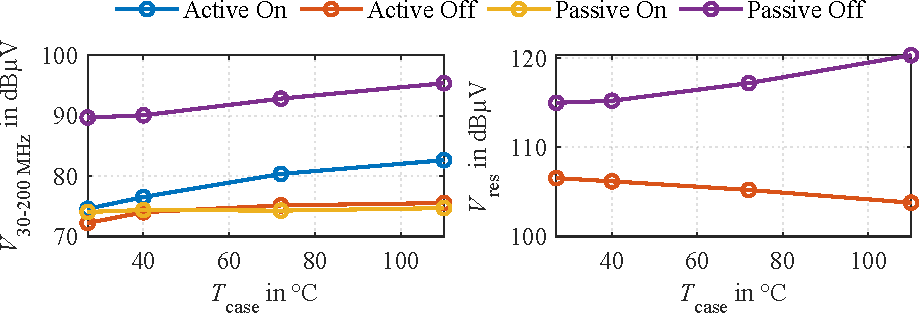
\includegraphics[scale = 1]{figures/7_MeasurementResults/MR_T_constE/MR_T_constE_Emission.pdf}
	\caption{Influence of the temperature on the EM emissions.}
	\label{fig:MR_T_constE_Emission}
\end{figure}

This is quantified in \fref{fig:MR_T_constE_Emission}, where the average FOM and the resonance peak value are plotted against the case temperature, separated for the active and passive device.
The active-off and passive-on transients show virtually no dependency on the case temperature, consistent with the negligible influence observed in the time- and frequency-domain results above.
In contrast, the passive-off transient, i.e., the reverse recovery of the freewheeling diode, shows the strongest temperature dependence among all four transients: the average FOM increases by approximately \SI{6}{dB} and the resonance peak value increases by approximately \SI{5}{dB} between \SI{27}{\celsius} and \SI{110}{\celsius}.

The active-on transient, which is only indirectly affected through the current overshoot imposed by the reverse-recovery current of the complementary device, follows the same trend, whereas the resonance peak value of the active-off transient even decreases slightly with increasing temperature.

Considering that this measurement covers only about half of the device's usable temperature range, the junction temperature must nonetheless be regarded as a strong contributor to the EM emissions, an influence that is almost exclusively mediated by the bipolar charge stored in the freewheeling diode.
This finding is particularly significant because the passive-off transient, whose temperature sensitivity is the strongest of all four transients, is already the dominant contributor to the overall EM emissions among all measurements presented in this thesis, even at room temperature.
The junction temperature must therefore be regarded as one of the most important parameters governing the EM emissions of a SiC MOSFET, and it deserves corresponding attention already at the converter design stage by including a temperature margin in the emission budget.

\FloatBarrier

\subsubsection*{Commutation-Loop Inductance}

Unlike the previous three parameters, the commutation-loop inductance \mi{L}{\sigma} is not a free design parameter that is tuned during the development phase to trade off against other requirements, but is always minimized as far as possible. 
It is determined by the physical layout of the power loop, e.g., by the parasitic inductance of the DC-link capacitors, the busbar or PCB traces, and the device packages, and can therefore only be reduced through the layout design.
Together with the output capacitance \mi{C}{oss} of the turned-off device, the commutation-loop inductance forms the resonant tank that is excited by every switching transient.
Increasing \mi{L}{\sigma} raises the characteristic impedance \mi{Z}{0} = \(\sqrt{\mi{L}{\sigma}/\mi{C}{oss}}\) of this tank, which increases the ringing amplitude for a given current excitation, while simultaneously lowering the resonant frequency \mi{f}{res} = $\sfrac{1}{2\pi\sqrt{\mi{L}{\sigma}\mi{C}{oss}}}$.
The commutation-loop inductance is therefore expected to primarily influence the overvoltage and the main resonance of both switching events, shifting it towards lower frequencies and increasing its amplitude, rather than to change the switching speed itself -- considering the speed is set to ensure constant switching losses across the sweep.

\begin{figure}[ht]
	\centering
	\begin{subfigure}[t]{\textwidth}
		\centering
		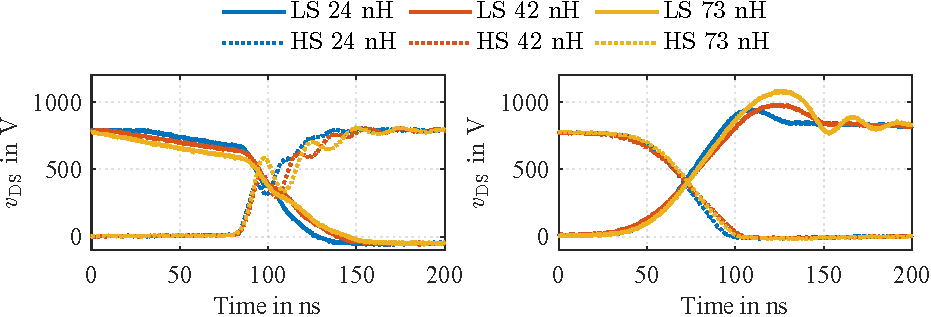
\includegraphics[scale = 1]{figures/7_MeasurementResults/MR_L_constE/MR_L_constE_Voltage_TD.pdf}
		\subcaption{Time-domain voltage measurement results.}
		\label{fig:MR_L_constE_Sweep_Voltage_TD}
	\end{subfigure} 
    
	\vspace{0.5cm}	
	
    \begin{subfigure}[t]{\textwidth}
		\centering
		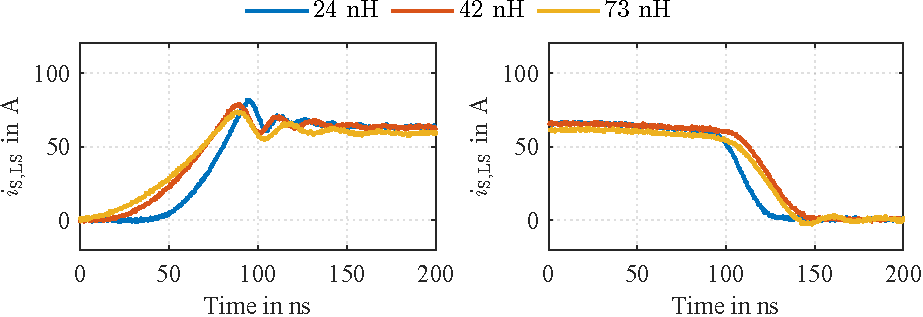
\includegraphics[scale = 1]{figures/7_MeasurementResults/MR_L_constE/MR_L_constE_Current_TD.pdf}
		\subcaption{Time-domain current measurement results.}
		\label{fig:MR_L_constE_Sweep_Current_TD}
	\end{subfigure}
	\caption{Time-domain results of the commutation-loop-inductance sweep.}
	\label{fig:MR_L_constE_Sweep_TD}
\end{figure}

Fig.~\ref{fig:MR_L_constE_Sweep_TD} shows the time-domain results of the commutation-loop-inductance sweep, covering \SI{24}{nH}, \SI{42}{nH}, and \SI{73}{nH}.
Because the gate resistance is co-adjusted for each inductance, the duration of the gate-controlled part of both the turn-on and the turn-off transient remains similar across the sweep.
The ringing that follows each transition, however, changes markedly: with increasing \mi{L}{\sigma}, the peak overvoltage after turn-off grows from \SI{940}{V} at \SI{24}{nH} to \SI{1080}{V} at \SI{73}{nH}, while the ringing frequency visibly decreases, consistent with the larger characteristic impedance and the lower resonant frequency of the \mi{L}{\sigma}-\mi{C}{oss} tank.
A similar, though less pronounced, trend is visible for the ringing excited during turn-on.

\begin{figure}[ht]
	\centering
	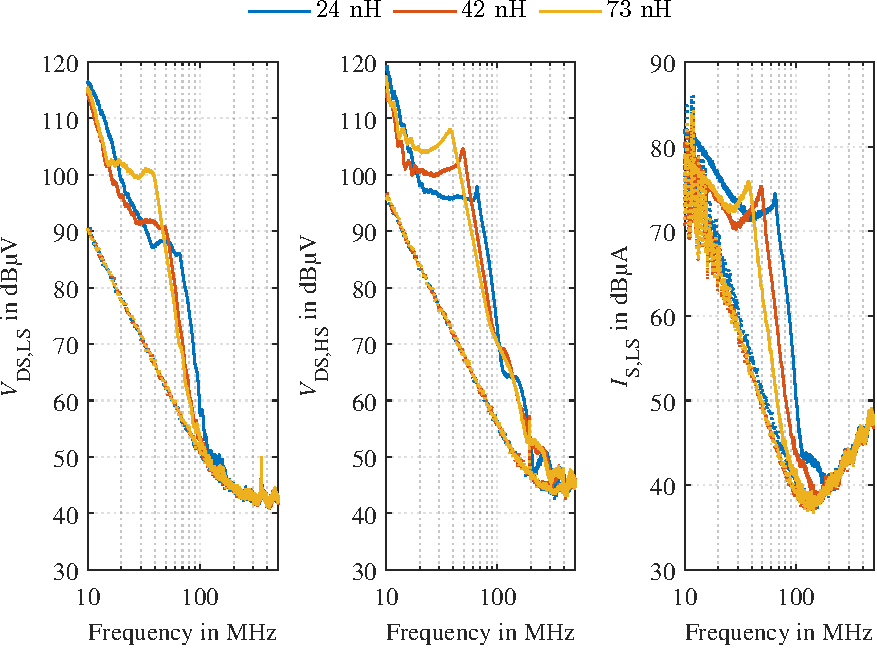
\includegraphics[scale = 1]{figures/7_MeasurementResults/MR_L_constE/MR_L_constE_FD.pdf}
	\caption{Frequency-domain measurement results of the commutation-loop-inductance sweep.}\label{fig:MR_L_constE_Sweep_FD}
\end{figure}

The corresponding frequency-domain spectra, shown in \fref{fig:MR_L_constE_Sweep_FD} and separated for the active and passive device as well as the commutation current, confirm this trend.
Below approximately \SI{10}{\mega\hertz}, the spectra of all three inductances coincide.
Towards higher frequencies, the spectra diverge: for \SI{24}{nH}, the main resonance appears at \SI{66}{\mega\hertz}, whereas for \SI{73}{nH} it shifts down to \SI{37}{\mega\hertz} and reaches a distinctly higher amplitude, in agreement with the lower resonant frequency and the larger characteristic impedance of the commutation loop.

\begin{figure}[ht]
	\centering
	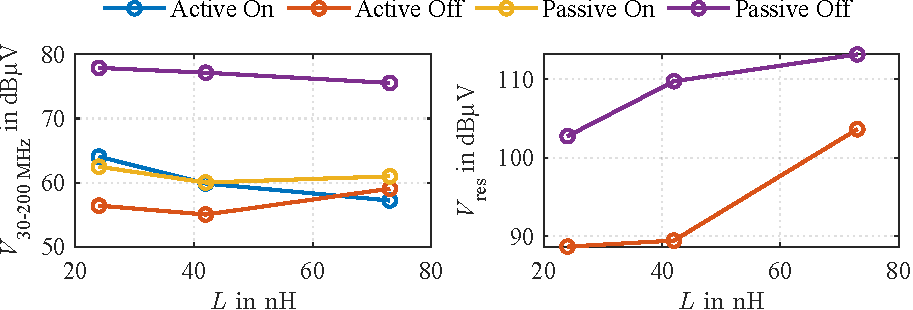
\includegraphics[scale = 1]{figures/7_MeasurementResults/MR_L_constE/MR_L_constE_Emission.pdf}
	\caption{Commutation-loop-inductance-dependent emission and loss analysis.}\label{fig:MR_L_constE_Emission}
\end{figure}

This is quantified in \fref{fig:MR_L_constE_Emission}, where the average FOM and the resonance peak value are plotted against the commutation-loop inductance, separated for the active and passive device and for turn-on and turn-off.
Interestingly, the average FOM does not follow the pronounced increase of the overvoltage observed in the time domain: the passive-off transient, which shows the highest average FOM of all four transients throughout the entire sweep, even decreases slightly, from \SI{78}{dB\micro V} to \SI{75.5}{dB\micro V}, the active-on transient decreases from \SI{64}{dB\micro V} to \SI{57}{dB\micro V}, and the active-off and passive-on transients remain within a narrow band of \SIrange{55}{61}{dB\micro V}.
This apparent contradiction is resolved by the resonance peak value: both the active-off and the passive-off resonance peak increase markedly with the commutation-loop inductance, by approximately \SI{15}{dB} and \SI{9}{dB}, respectively.
The reason is that increasing \mi{L}{\sigma} does not add emission energy, but merely shifts it from higher to lower frequencies, following the falling resonant frequency of the \mi{L}{\sigma}-\mi{C}{oss} tank; such a shift within the averaging window is what the spectral average cannot capture, since it weighs all frequencies within its \SIrange{30}{200}{\mega\hertz} range equally, regardless of where the emissions actually occur.
This highlights an important limitation of a fixed-band average FOM.

Although increasing \mi{L}{\sigma} thereby lowers the emissions at higher frequencies, this seems very unlikely to ever be exploited deliberately as a means to reduce EM emissions, since it comes at the cost of both increased low-frequency emissions and a higher overvoltage.
Since \mi{L}{\sigma} is fixed by the power-stage layout rather than by the gate driver or the device, this influence cannot be corrected during operation; it must therefore be addressed already during the layout design of the commutation loop, for instance by minimizing the enclosed loop area and by placing the DC-link capacitors as close as possible to the switching devices.
%!TeX root = main.tex
%!encoding = UTF-8 Unicode
\subsection{Influence of MOSFET Parameters}
\label{sec:MR_MOSFET}

This section examines the influence of parameters that are determined by the device engineer during MOSFET design, rather than by the application engineer during converter design.
In principle, the presented measurement methodology could be used to investigate more fundamental design-of-experiment parameters, such as the doping concentration, the cell pitch, or the gate-oxide thickness, that are typically only accessible to the device engineer.
However, since the presented measurement setup is built around the D2PAK package, only packaged chips can be currently measured, rather than dedicated engineering samples with such tailored design variations, which normally come as bare-dies on various adapter PCBs.
Consequently, this section is limited to those parameters that vary among commercially available finished products, namely the active chip area, reflected in the current rating, the SiC technology generation within Bosch's own device portfolio, and the semiconductor manufacturer.
The active chip area and the SiC technology generation directly affect the intrinsic switching behavior, and unlike the external parameters discussed in Section~\ref{sec:MR_External}, they cannot be tuned by the application engineer once a device has been selected.
For each of these two parameters, a comparison is performed while the switching losses are kept constant, so that the differences observed in the frequency-domain spectra can be attributed to the parameter itself rather than to a shift in the switching speed.

\subsubsection*{Active Chip Area}

To investigate the influence of the active chip area, three devices from the same Bosch SiC MOSFET generation with active areas of \SI{5}{mm^2}, \SI{8}{mm^2}, and \SI{11}{mm^2} are compared.
Because the current rating of a MOSFET scales approximately with its active area, so do most of the underlying device parameters: the parasitic capacitances \mi{C}{oss}, \mi{C}{iss}, and \mi{C}{rss}, the channel transconductance \mi{g}{m} evaluated at the nominal current, and the reverse-recovery charge \mi{Q}{rr} of the intrinsic body diode all increase roughly linearly with the active area, since a larger die simply places more of the same unit cells in parallel.
By contrast, parameters that are set by the vertical doping profile and the gate-oxide process rather than by the lateral cell count, most notably the threshold voltage \mi{V}{th} and the blocking-voltage rating \mi{V}{(BR)DSS}, remain essentially unaffected by the active area.

Since the load current cannot be scaled together with the chip area for this comparison, all three devices are switched at the same absolute load current of \mi{I}{L} = \SI{30}{A}.
As a consequence, and because the nominal current rating \mi{I}{N} differs between the compared devices (\SI{30}{A}, \SI{45}{A}, and \SI{60}{A}  for the \SI{5}{mm^2}, \SI{8}{mm^2}, and \SI{11}{mm^2} chips), the three devices are not operated at the same relative operating point: the smallest chip is loaded to approximately \mi{I}{N}, whereas the largest chip is loaded to only approximately \mi{I}{N}/2.
This distinction matters because some of the relevant device parameters, most notably the transconductance, are inherently nonlinear in the drain current, so that part of the differences observed below reflects this shift in the relative operating point in addition to the active area itself.

\begin{figure}[ht]
	\centering
	\begin{subfigure}[t]{\textwidth}
		\centering
		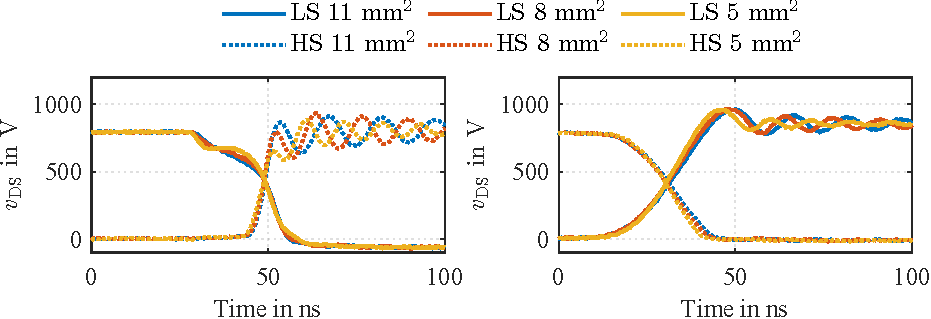
\includegraphics[scale = 1]{figures/7_MeasurementResults/MR_A_constE/MR_A_constE_Voltage_TD.pdf}
		\subcaption{Time-domain voltage measurement results.}
		\label{fig:MR_A_constE_Sweep_Voltage_TD}
	\end{subfigure} 
    
	\vspace{0.5cm}	
	
    \begin{subfigure}[t]{\textwidth}
		\centering
		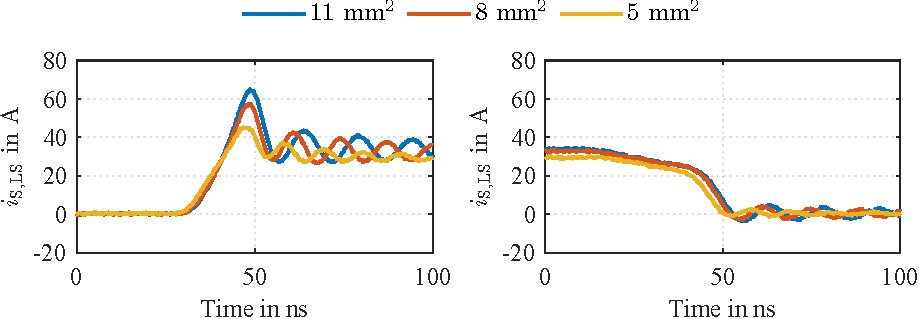
\includegraphics[scale = 1]{figures/7_MeasurementResults/MR_A_constE/MR_A_constE_Current_TD.pdf}
		\subcaption{Time-domain current measurement results.}
		\label{fig:MR_A_constE_Sweep_Current_TD}
	\end{subfigure}
	\caption{Time-domain results of the active-chip-area sweep.}
	\label{fig:MR_A_constE_Sweep_TD}
\end{figure}

Fig.~\ref{fig:MR_A_constE_Sweep_TD} shows the time-domain results of the active-chip-area sweep.
The steady-state current after each transient is, as intended, virtually identical for all three devices, since it is set by the common load current.
During turn-on, however, the current peak of the passive device increases markedly with the active area, from approximately \SI{45}{A} at \SI{5}{mm$^2$} to approximately \SI{65}{A} at \SI{11}{mm$^2$}, consistent with the larger output capacitance of the larger chip discussed above.
During turn-off, all three devices reach a comparable peak overvoltage, but the larger chips exhibit a visibly stronger ringing pattern than the smallest one, which is analyzed more quantitatively in the frequency domain below.

\begin{figure}[ht]
	\centering
	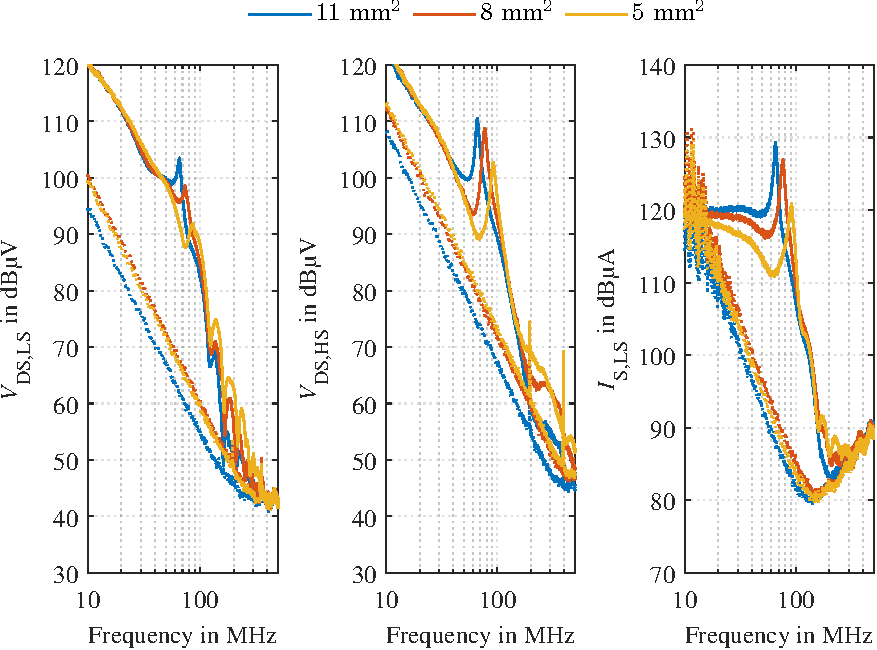
\includegraphics[scale = 1]{figures/7_MeasurementResults/MR_A_constE/MR_A_constE_FD.pdf}
	\caption{Frequency-domain measurement results of the active-chip-area sweep.}\label{fig:MR_A_constE_Sweep_FD}
\end{figure}

The corresponding frequency-domain spectra, shown in \fref{fig:MR_A_constE_Sweep_FD}, confirm this trend: a resonance is visible in both device voltages and the commutation current, shifting from \SI{92}{MHz} for the smallest chip to \SI{65}{MHz} for the biggest chip, consistent with the expected $\mi{f}{res} \propto 1/\sqrt{\mi{C}{oss}}$ scaling given the roughly twofold increase in \mi{C}{oss} between the two devices.
The resonance amplitude likewise increases clearly with the active area, in agreement with the larger output capacitance discussed above.
At higher frequencies, by contrast, the trend reverses: the broadband emissions of the \SI{11}{mm^2} chip are up to \SI{10}{dB} smaller than those of the smallest chip, for both the active and the passive device, showing a massive impact of the active area on the spectral content of the switching transients.

\begin{figure}[ht]
	\centering
	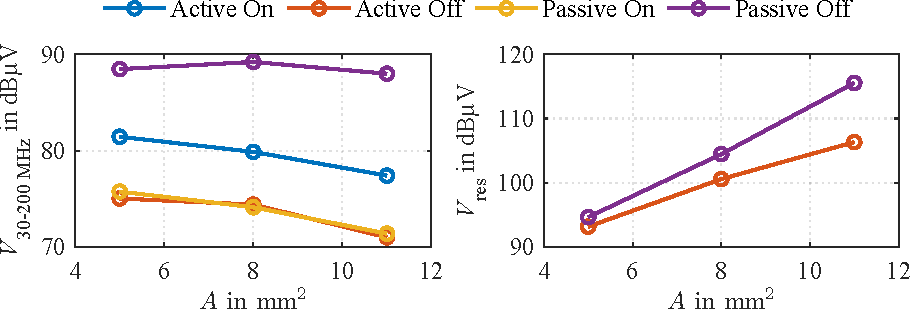
\includegraphics[scale = 1]{figures/7_MeasurementResults/MR_A_constE/MR_A_constE_Emission.pdf}
	\caption{Active-chip-area-dependent emission analysis.}
	\label{fig:MR_A_constE_Emission}
\end{figure}

This is quantified in \fref{fig:MR_A_constE_Emission}, where the average FOM and the resonance peak value are plotted against the active area, separated for the active and passive device.
As with the commutation-loop inductance, the average FOM does not follow the trend of the resonance peak: the active-on transient decreases from approximately \SI{81.5}{dB\micro V} to \SI{77.5}{dB\micro V}, the active-off and passive-on transients decrease similarly, from approximately \SI{75}{dB\micro V} to \SI{71.5}{dB\micro V}, and the passive-off transient remains virtually constant at approximately \SIrange{88}{89}{dB\micro V}.
In contrast, the resonance peak value increases markedly with the active area for both turn-off transients: the active-off resonance peak increases from approximately \SI{93}{dB\micro V} to \SI{106}{dB\micro V}, and the passive-off resonance peak, the most sensitive of the two, increases from approximately \SI{95}{dB\micro V} to \SI{115.5}{dB\micro V}, an increase of more than \SI{20}{dB} over the studied range.
As for the commutation-loop inductance, this apparent contradiction is resolved by a shift of the resonance towards lower frequencies: because \mi{C}{oss} increases with the active area, the resonant frequency of the \mi{L}{\sigma}-\mi{C}{oss} tank falls from \SI{92}{MHz} to \SI{65}{MHz}, as shown above, moving part of the emitted energy from the upper to the lower end of the \SIrange{30}{200}{MHz} averaging window; since the spectral average weighs all frequencies within this range equally, such a shift is not captured, even though the resonance peak itself grows substantially.
This effect is reinforced by the broadband emissions: because the larger Miller capacitance of a bigger chip slows down the switching transient, as already discussed in Section~\ref{sec:MR_External} for the gate resistance, the broadband spectral content away from the resonance additionally decreases with the active area, further lowering the spectral average.

Since the active chip area is primarily selected by the application engineer to meet the required current rating of the converter, rather than to trade off EM emissions, this sensitivity is best understood as a design consequence rather than a free parameter: oversizing a device beyond the current rating strictly required by the application carries a hidden cost in the form of a markedly higher resonance peak, even though the broadband average FOM would, if anything, suggest the opposite trend.

\FloatBarrier

\subsubsection*{SiC Device Technology}

To highlight the influence of the device structure on the EM emissions, two devices from the first and second SiC MOSFET generation of the Robert Bosch SiC MOSFET portfolio are selected, matched in package, voltage rating, and current rating, and compared while the switching-loss energies are again matched between the two devices.
The specific design and process changes made between the two generations are proprietary and are therefore not disclosed in this work; rather than a root-cause analysis, this comparison is intended as a demonstration of what the presented measurement methodology can reveal about device improvements, and thus serves as a teaser for the potential of power device optimization for EM emission reduction.
Beyond this comparison within Bosch's own device history, Section~\ref{sec:benchmark} extends the analysis to a comparative benchmarking across different semiconductor manufacturers, spanning the wider SiC MOSFET market.

\begin{figure}[ht]
	\centering
	\begin{subfigure}[t]{\textwidth}
		\centering
		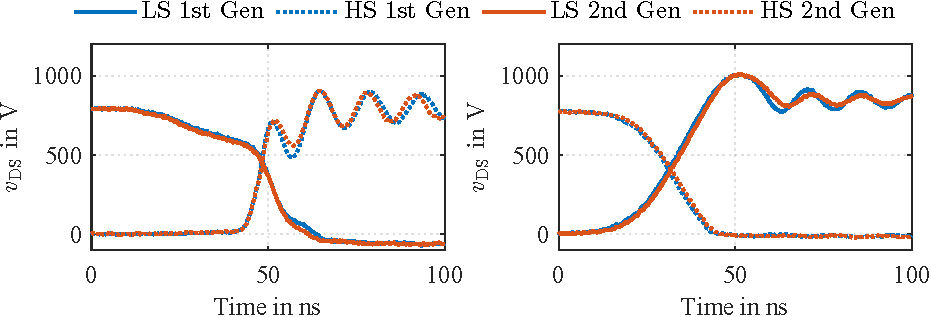
\includegraphics[scale = 1]{figures/7_MeasurementResults/MR_Gen_constE/MR_Gen_constE_Voltage_TD.pdf}
		\subcaption{Time-domain voltage measurement results.}
		\label{fig:MR_Gen_constE_Sweep_Voltage_TD}
	\end{subfigure} 
    
	\vspace{0.3cm}	
	
    \begin{subfigure}[t]{\textwidth}
		\centering
		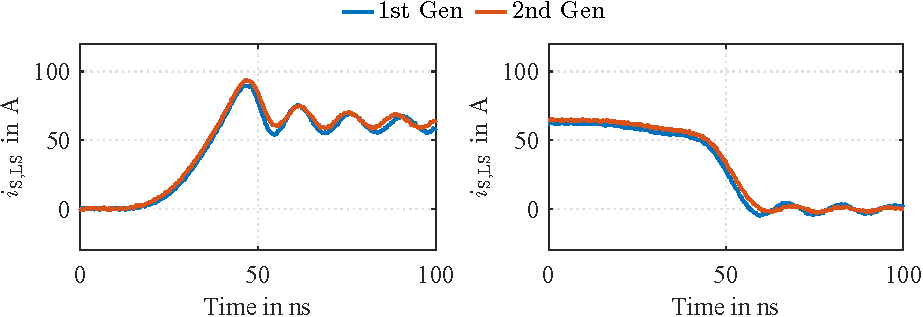
\includegraphics[scale = 1]{figures/7_MeasurementResults/MR_Gen_constE/MR_Gen_constE_Current_TD.pdf}
		\subcaption{Time-domain current measurement results.}
		\label{fig:MR_Gen_constE_Sweep_Current_TD}
	\end{subfigure}
	\caption{Time-domain results of the SiC-technology-generation sweep.}
	\label{fig:MR_Gen_constE_Sweep_TD}
\end{figure}

Fig.~\ref{fig:MR_Gen_constE_Sweep_TD} shows the corresponding time-domain waveforms.
The overall switching trajectories of both generations are very similar, consistent with the closely matched switching-loss energies targeted by this comparison; the most visible difference appears in the post-transient ringing, where the two generations settle with a visibly different ringing frequency and damping, foreshadowing the different resonance behavior observed in the frequency domain below.

\begin{figure}[ht]
	\centering
	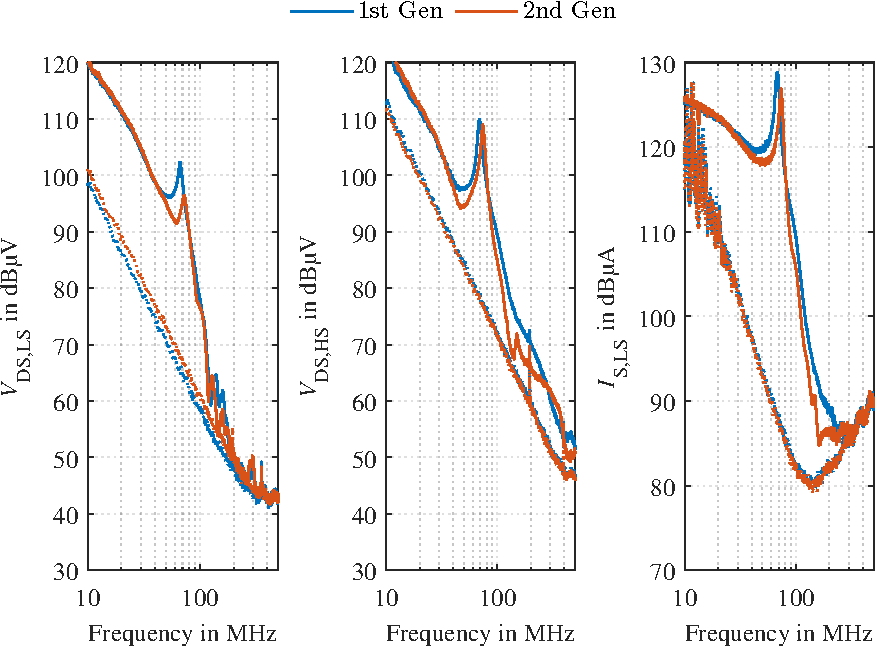
\includegraphics[scale = 1]{figures/7_MeasurementResults/MR_Gen_constE/MR_Gen_constE_FD.pdf}
	\caption{Frequency-domain measurement results of the SiC-technology-generation sweep.}\label{fig:MR_Gen_constE_Sweep_FD}
\end{figure}

The corresponding frequency-domain spectra, shown in \fref{fig:MR_Gen_constE_Sweep_FD}, reveal a more substantial difference between the two generations than was visible in the time domain.
In both device voltages, the second generation shows a lower resonance peak than the first generation, by roughly \SI{7}{dB} in \mi{V}{DS,LS} (from approximately \SI{102}{dB\micro V} to \SI{96}{dB\micro V}) and by roughly \SI{2}{dB} in \mi{V}{DS,HS} (from approximately \SI{110}{dB\micro V} to \SI{108}{dB\micro V}).
The broadband behavior of the active device remains the same between the two generations, while the broadband content of the passive device decreases by up to \SI{9}{dB} in the second generation, consistent with the lower resonance peak.
Interestingly, the second generation shows a small second resonance at \SI{149}{MHz} in the high-side voltage, which is absent in the first generation.
This is apparent in all measurements and increases with higher temperatures, suggesting that it is a real effect rather than a measurement artifact, but its origin cannot be traced back to a specific root cause in this work.

In the commutation current, the second generation shows a similar improvement: the resonance peak decreases by roughly \SI{3}{dB}, from \SI{87}{dB\micro A} to \SI{84}{dB\micro A}, and the broadband content away from the resonance decreases by up to \SI{6}{dB}, consistent with the improvement already observed for the device voltages.
This consistent improvement across both device voltages and the commutation current suggests that the underlying technology change benefits the switching transient broadly, rather than trading off one metric against another.

\begin{figure}[ht]
	\centering
	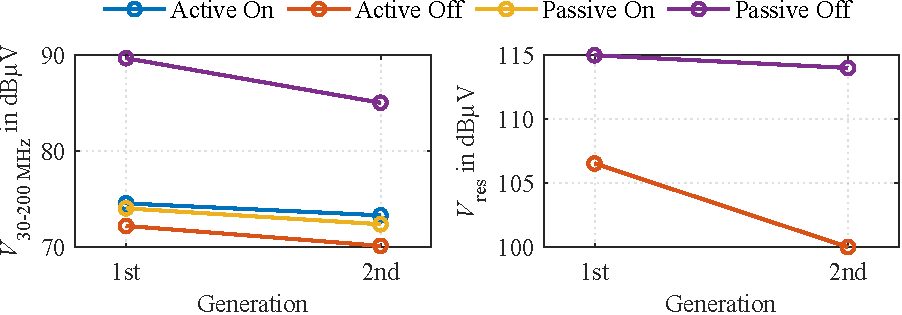
\includegraphics[scale = 1]{figures/7_MeasurementResults/MR_Gen_constE/MR_Gen_constE_Emission.pdf}
	\caption{SiC-technology-generation-dependent emission analysis.}
	\label{fig:MR_Gen_constE_Emission}
\end{figure}

This is quantified in \fref{fig:MR_Gen_constE_Emission}, where the average FOM and the resonance peak value of the device voltages are plotted for both generations.
The average FOM improves slightly but consistently from the first to the second generation for all four transients, most notably for the passive-off transient, which decreases from approximately \SI{89.5}{dB\micro V} to \SI{85}{dB\micro V}, while the remaining three transients improve by roughly \SIrange{1}{2}{dB}.
The resonance peak value improves even more markedly for the active-off transient.
Taken together, unlike for the active chip area in the previous subsection, the second generation improves both the average FOM and the resonance peak of the device voltages, without a trade-off between the two metrics.

Since the underlying design and process changes between the two generations are not disclosed here, this comparison cannot be traced back to a specific root cause.
Nevertheless, it demonstrates that a considerable improvement in EM emissions, up to \SI{15}{dB} in the resonance peak, can be achieved purely through technology development, without any change to the application circuit; the presented measurement methodology thus provides device engineers with direct, quantitative feedback on the EM-emission impact of such technology changes, in addition to the classical figures of merit such as on-resistance and switching losses.

\FloatBarrier


\subsubsection*{Benchmarking of SiC MOSFET Manufacturers}
\label{sec:benchmark}
Having examined the active chip area and the SiC technology generation, this final subsection turns to a last approach to highlight device influence: the semiconductor manufacturer.
Unlike the chip-area and technology-generation comparisons, which isolate the parameter of interest by matching a single switching-loss operating point, comparing manufacturers at just one such point would conflate the parameter under study with each device's individual loss-emission trade-off; instead, this comparison spans the entire trade-off curve of each device.
For this purpose, four \SI{1200}{V} SiC MOSFETs in D2PAK packages from different manufacturers, matched in current rating to $\SI{60}{A}\pm\SI{5}{A}$, are compared, operated at $\mi{V}{DC}~=~\SI{800}{V}$ and $\mi{I}{L}~=~\SI{60}{A}$ at room temperature.
To trace out this trade-off curve for each device, a gate-resistance sweep of $\mi{R}{G,ext} = [1, 5, 10, 20, 30, 50]~\si{\ohm}$ is performed, with an overvoltage limit of \SI{1200}{V} as the stopping criterion.
For each operating point, the average FOM is calculated for the active and passive switch voltages, together with the switching-loss energy \mi{E}{sw,tot}.

\begin{figure}[h]
	\centering
	\input{7_MeasurementResults/MR_MarketOverview.tex}
	\caption{Comparative analysis of EM noise emission performance for SiC MOSFETs from different manufacturers.}
	\label{fig:MR_CompetitorAnalysis}
\end{figure}

The resulting comparison, plotted in \fref{fig:MR_CompetitorAnalysis}, confirms the expected trend of increasing average FOM with decreasing switching-loss energy for all four devices.
However, at a given switching-loss energy, the four devices do not trade off losses for EM emissions equally well: at the lowest switching-loss energy of approximately \SI{0.7}{mJ}, the four devices emit within roughly \SI{2.5}{dB} of each other, whereas at the highest switching-loss energy of \SI{3.25}{mJ}, the spread widens to up to \SI{7}{dB}, driven primarily by one device trading off losses for EM emissions markedly worse than the other three.
When this is compared to the sensitivity of the average FOM to the external parameters discussed in Section~\ref{sec:MR_External}, where a change of \SI{5}{dB} was observed for a change of \SI{10}{nH} in the commutation-loop inductance, it becomes clear that the choice of semiconductor technology can have a similar or even larger impact on EM emissions than the layout design of the commutation loop.
This establishes EM noise emission as an additional design dimension alongside the classical trade-off between switching and conduction losses, and demonstrates the capability of the introduced measurement environment to benchmark competing semiconductor technologies on this basis.

\FloatBarrier
%!TeX root = main.tex
%!encoding = UTF-8 Unicode
\subsection{Summary of Measurement Studies}
\label{sec:MR_Summary}

Building on the individual comparisons discussed in Sections~\ref{sec:MR_External} and~\ref{sec:MR_MOSFET}, this final section condenses the influence of all investigated parameters into a single, compact overview.
For each parameter, a linear sensitivity of the average FOM is derived from the measured data, separately for the active-off and passive-off transients, since these two switching events are, according to the discussions above, the dominant contributors to the overall EM emissions.
Table~\ref{tab:SummaryMRStudies} reports this sensitivity for three different measurement constraints: constant gate resistance (Const. \mi{R}{G}), constant peak overvoltage (Const. OV), and constant switching-loss energy (Const. \mi{E}{sw}); the latter is the constraint discussed throughout the main text of this chapter, while the former two are documented only in Appendix~\ref{app:additional_measurements} but are included here for completeness.
The gate resistance itself is the only parameter for which no such constraint applies, since it is the swept quantity itself rather than a co-adjusted compensation variable; its sensitivity is therefore reported directly in \si{dB/\ohm}, as well as related to the switching-loss energy it trades off, in \si{dB/mJ}, which quantifies the cost, in terms of EM emissions.

\begin{table}[ht]
	\caption{Summary of the impact of different parameters on the active-off and passive-off measurement results.}
	\label{tab:SummaryMRStudies}
	\centering
	\setlength{\tabcolsep}{18pt}
	\begin{tabular}{@{}lccl@{}}
		\toprule
		\textbf{Parameter} & \textbf{Active Off} & \textbf{Passive Off} & \textbf{Condition} \\
		\midrule
		\multirow{2}{*}{Gate drive} & -0.56 dB/$\Omega$ & -0.39 dB/$\Omega$ & \mi{R}{G} sweep \\
		                            & -14.53 dB/mJ & -9.88 dB/mJ & \mi{R}{G} sweep \\
		\midrule
		\multirow{3}{*}{Chip Size $A$} & -0.92 dB/mm & -0.59 dB/mm  & Const. \mi{R}{G} \\
		                    & -0.92 dB/mm  & -0.38 dB/mm  & Const. OV \\
		                    & -0.67 dB/mm  & -0.08 dB/mm  & Const. \mi{E}{sw} \\
		\midrule
		\multirow{3}{*}{\shortstack[l]{Neg. Driver Supply\\\mi{V}{ee,driver}}} & -0.67 dB/V & -0.47 dB/V & Const. \mi{R}{G} \\
		                                      & +0.08 dB/V & +0.23 dB/V & Const. OV \\
		                                      & -0.15 dB/V & -0.29 dB/V & Const. \mi{E}{sw} \\
		\midrule
		\multirow{3}{*}{Temperature $T$} & 0.005 dB/K & 0.064 dB/K & Const. \mi{R}{G} \\
		                    & 0.003 dB/K & 0.013 dB/K & Const. OV \\
		                    & 0.035 dB/K & 0.071 dB/K & Const. \mi{E}{sw} \\
		\midrule
		\multirow{3}{*}{\shortstack[l]{Commutation-Loop\\ Inductance \mi{L}{\sigma}}} & 0.09 dB/nH & 0.01 dB/nH & Const. \mi{R}{G} \\
		                              & -0.41 dB/nH & -0.12 dB/nH & Const. OV \\
		                              & 0.06 dB/nH & -0.05 dB/nH & Const. \mi{E}{sw} \\
		\midrule
		\multirow{3}{*}{Bosch Generation} & +3 dB/Gen & -4.5 dB/Gen & Const. \mi{R}{G} \\
		                                  & -3.5 dB/Gen & -2.9 dB/Gen & Const. OV \\
		                                  & -2.1 dB/Gen & -4.6 dB/Gen & Const. \mi{E}{sw} \\
		\bottomrule
	\end{tabular}
\end{table}

Because these sensitivities are expressed per unit of each parameter, and the physically or economically accessible range of each parameter differs enormously from one another, from a single manufacturing step for the SiC technology generation to a swing of more than \SI{100}{K} for the junction temperature, the raw slopes reported in Table~\ref{tab:SummaryMRStudies} must not be compared directly across parameters to rank their importance: a numerically large sensitivity per generation, for instance, is not automatically more relevant in practice than a numerically small sensitivity per kelvin, once it is considered that the accessible temperature swing is more than two orders of magnitude larger than the single generation step it would otherwise be compared to.
A fair comparison instead requires weighting each sensitivity by the range over which the corresponding parameter can realistically vary in an application; \tref{tab:SummaryMRStudiesRange} performs this weighting explicitly, by multiplying the constant-\mi{E}{sw} sensitivity of each parameter, or, for the gate resistance, its raw sensitivity in \si{dB/\ohm}, since no such constraint applies to it, with the full practically relevant range of that parameter, thereby reporting the maximum achievable change in the average FOM over the entire operating range.
The present table is therefore best used to compare a given parameter across the three measurement constraints, rather than to compare different parameters against each other.

\begin{table}[ht]
	\caption{Maximum change in average FOM over the full practical operating range of each parameter, obtained by scaling the constant-\mi{E}{sw} sensitivities of \tref{tab:SummaryMRStudies} with the stated operating range.}
	\label{tab:SummaryMRStudiesRange}
	\centering
	{%
	\renewcommand{\tabularxcolumn}[1]{>{\centering\arraybackslash}m{#1}}
	\begin{tabularx}{\textwidth}{@{}>{\raggedright\arraybackslash}XXXX@{}}
		\toprule
		\textbf{Parameter} & \textbf{Operating Range} & \textbf{Active Off} & \textbf{Passive Off} \\
		\midrule
		Gate resistance \mi{R}{G} & \SIrange{1}{50}{\ohm} & -27.4 dB & -19.1 dB \\
		Active chip area $A$ & \SIrange{5}{50}{mm^2} & -30.2 dB & -3.6 dB \\
		Neg. driver supply \mi{V}{ee,driver} & \SIrange{-10}{0}{V} & -1.5 dB & -2.9 dB \\
		Temperature $T$ & \SIrange{25}{175}{\celsius} & +5.3 dB & +10.7 dB \\
		Inductance \mi{L}{\sigma} & \SIrange{5}{100}{nH} & +5.7 dB & -4.8 dB \\
		Bosch generation & 1 -- 2 & -2.1 dB & -4.6 dB \\
		\bottomrule
	\end{tabularx}
	}
\end{table}

Over their full practical operating ranges, the gate resistance and the active chip area emerge as the two parameters with by far the largest achievable impact on the average FOM, at approximately \SI{-27}{dB} to \SI{-30}{dB} for the active-off transient, whereas the SiC technology generation and the negative gate-driver bias, whose accessible range is inherently limited to a single manufacturing step and to a few volts, respectively, remain confined to a few decibels even at their extreme settings.
The junction temperature and the commutation-loop inductance fall in between, each capable of shifting the average FOM by roughly \SIrange{5}{11}{dB} across their full practical range, despite their comparatively modest per-unit sensitivities in \tref{tab:SummaryMRStudies}.
It must be emphasized that these figures are obtained by linearly extrapolating the fitted sensitivities beyond the narrower ranges that were actually measured for some parameters, most notably the chip area, the temperature, and the commutation-loop inductance, and should therefore be interpreted as first-order estimates of the maximum achievable impact rather than as validated measurement results; in particular, nonlinear effects such as the measurement noise floor at low emission levels, discussed for the gate resistance in Section~\ref{sec:MR_External}, are not captured by this linear extrapolation and may cause the true achievable change to deviate from the values reported here.

Comparing the three measurement constraints further reveals that the sign and magnitude of a parameter's apparent sensitivity can depend strongly on which other quantity is held constant: the negative gate-driver bias, for instance, decreases the average FOM under constant gate resistance and constant switching-loss energy, but increases it under constant overvoltage, and the SiC technology generation even reverses sign for the active-off transient between the constant-\mi{R}{G} and the constant-\mi{E}{sw} conditions.
This sensitivity to the chosen constraint confirms, once more, the central premise of this chapter: any statement about the EM-emission impact of a single parameter is only meaningful once the quantities that are held constant, or allowed to vary, alongside it are clearly specified.

Taken together, this summary demonstrates that the measurement methodology and the spectral FOM framework developed in this thesis can not only characterize the EM emissions of a single device or converter, but also quantify and rank the often competing physical mechanisms that govern these emissions across a wide range of design and operating parameters, providing both the converter designer and the device engineer with a quantitative basis for weighing EM performance against the classical trade-offs of switching losses and blocking-voltage margin.



